%!TEX root = ../thesis.tex
%*******************************************************************************
%****************************** Optim2D Chapter ********************************
%*******************************************************************************
\chapter{L-BFGS Optimisation of Phase-Only Hologram}
\label{chapter:L-BFGS Optimisation of Phase-Only Hologram}

\graphicspath{{Chapter_Optim_CGH/Figs/}}

\textit{Note: Parts of this chapter have been published in Ref. \cite{Sha2022,Sha2023}}\\\\


As previously introduced in \cref{chapter:Literature Review}, currently available spatial light modulators (SLMs) can only modulate either phase or amplitude, so algorithms are needed to compute amplitude-only or phase-only holograms, among which the phase-only holograms are usually preferred due to their higher energy efficiency, leading to the emergence of the classical phase retrieval algorithms reviewed in \cref{sec:cgh}. With the developments in modern numerical optimisation methods and computational power, advances in CGH algorithms can be made. A search in the literature has found some recent work generating CGH using numerical optimisation methods \cite{Zhang2017, Liu2020, Choi2021, Chen2021}. This chapter therefore implements the use of numerical optimisation methods for hologram generation, including the novel method using the L-BFGS optimiser to compute phase-only holograms. The following sections start from the background knowledge of numerical optimisation including L-BFGS algorithm, which also serves as the theoretical background for \cref{chapter:Multi Frame Holograms Batched Optimisation}, then introduces and carries out the optimisation of phase hologram.



\section{Numerical Optimisation Methods} \label{sec:Numerical Optimisation Methods}

\subsection{Optimisation framework} \label{sec:Optimisation framework}
Numerical optimisation methods aim to find an optimal solution which minimise an objective function numerically. They begin with an initial guess of the optimal solution ($\textbf{x}_{0}$) and then, after iterations, generate a sequence of gradually improved estimates until they reach a solution \cite{Nocedal2006}. If we have $\textbf{x}$ as the vector of variables, and denote $f(\textbf{x})$ as the objective function, which is a function of $x$ we want to minimise, any unconstrained optimisation problem can be written as:
\begin{equation}
  \underset{\textbf{x}\in R^n}{\text{minimise}}\quad f(\textbf{x})
  \label{eq:minimise_F}
\end{equation}

Numerical optimisation then calculate the optimal solution $\textbf{x}^*$ iteratively, the iteration is given by:
\begin{equation}
  \textbf{x}_{k+1} = \textbf{x}_k+\alpha_k \textbf{p}_k
  \label{eq:optimisation_iteration}
\end{equation}
where the positive scalar $\alpha_k$ is called step length, or sometimes may be referred as `learning rate' in some context, and the vector $\textbf{p}_k$ is the search direction, which usually takes the form of
\begin{equation}
  \textbf{p}_k = -\textbf{B}_k^{-1} \nabla f_{k} \label{eq:general-descent-direction}
\end{equation}
where $\textbf{B}_k$ is a nonsingular matrix that varies for different optimisation methods, and $\nabla f_k$ is the gradient, which, if unable to evaluate directly, can be approximated by:
\begin{align}
  \nabla f_k         & \approx \frac{f_{k+1}-f_{k}}{\textbf{x}_{k+1}-\textbf{x}_{k}} \nonumber \\
  \text{where}\  f_k & \ \text{denotes}\  f(\textbf{x}_k)
\end{align}

The strategy used to determine $\textbf{p}_k$ distinguishes one algorithm from another. Most methods make use of the values of $f$, $\nabla f$ and $\nabla^2 f$, and some methods even make use of the accumulated historical values of those derivatives, which are further discussed in \cref{sec:GD} - \cref{sec:L-BFGS}.


\subsection{Gradient Descent}\label{sec:GD}
Gradient descent (GD) is a first-order optimisation method, it finds a local minimum by following the negative of the gradient (i.e. the steepest descent direction). The $\textbf{B}_k$ (in \cref{eq:general-descent-direction}) for gradient descent simply takes the value of $\textbf{I}$, which is the identity matrix. And the search direction becomes:
\begin{equation}
  \textbf{p}_k = -\nabla f_k
\end{equation}
The steepest descent method is very intuitive: among all possible directions to move away from $\textbf{x}_{k}$, the steepest gradient direction is the one which $f$ decreases most rapidly. The advantage of this method is that it requires few computation and memory resource, because it only requires a computation of the first derivative, and it does not require any accumulation of historical gradients. However, it is a greedy method that only considers the current iteration without any global consideration, so it can be extremely slow on complicated problems. \cite{Nocedal2006}

To work around the disadvantage, a few variants have emerged, such as AdaGrad \cite{Duchi2011}, RMSProp \cite{Tieleman2012} and Adam \cite{Kingma2015} which combines the advantages of AdaGrad and RMSProp. The Adam method is an iconic variant of GD, often referred to as `gradient descent with momentum', as the name Adam is derived from `adaptive moment estimation'. Adam algorithm is based on adaptive estimates of lower-order moments \cite{Kingma2015}. It computes individual adaptive learning rates for different parameters from estimates of first and second moments of the gradients \cite{Kingma2015}.


\subsection{Newton's Method}
Newton's method is a second-order optimisation method. Its search direction is derived from the second-order Taylor series approximation to $f(\textbf{x}_k+\textbf{p})$, which is
\begin{equation}
  f(\textbf{x}_k+\textbf{p}) \approx f_k + \textbf{p}^T \nabla f_k + \frac{1}{2}\textbf{p}^T \nabla^2 f_k \textbf{p} \stackrel{\text{def}}{=}m_k(\textbf{p})
\end{equation}
The Newton direction can then be obtained by finding the vector $\textbf{p}$ that minimises $m_k(\textbf{p})$. By setting the derivative of $m_k(\textbf{p})$ to zero, $\textbf{p}$ can be obtained as:
\begin{equation}
  \textbf{p}_k=-\nabla^2 f_k^{-1}\nabla f_k \label{eq:Newton-direction}
\end{equation}
By comparing \cref{eq:Newton-direction} to \cref{eq:general-descent-direction}, it can be seen that the Newton's method has a $\textbf{B}_k$ of $\nabla^2 f_k$. Unlike the gradient descent method, there is a "natural" step length of 1 associated with the Newton direction, so $\alpha_k = 1$ by default and is only adjusted when it does not produce a satisfactory reduction in the value of $f$.

The Newton direction is reliable when the difference between the true function $f(\textbf{x}_k+\textbf{p})$ and its quadratic model $m_k(\textbf{p})$ is not too large. Methods that use the Newton direction have a fast rate of local convergence, typically quadratic. After a neighbourhood of the solution is reached, convergence to high accuracy often occurs in just a few iterations. The main drawback of the Newton direction is the need for the Hessian $\nabla^2 f_k$. Explicit computation of this matrix of second derivatives can sometimes be a cumbersome, error-prone, and expensive process. \cite{Nocedal2006}


\subsection{Quasi-Newton Method}\label{sec:BFGS}
Quasi-Newton method provides an attractive alternative to Newton's method, in that they do not require computation of the Hessian and yet still attain a super linear rate of convergence. In place of the true Hessian $\nabla^2 f_k$, they use an approximation $\mathcal{H}_k \stackrel{\text{def}}{=} \textbf{B}_k^{-1}$, which is updated after each step to take account of the additional knowledge gained during the step. The updates make use of the fact that changes in the gradient provide information about the second derivative of $f$ along the search direction. The most popular quasi-Newton algorithm is the Broyden-Fletcher-Goldfarb-Shanno (BFGS) method, named for its discoverers Broyden, Fletcher, Goldfarb, and Shanno. \cite{Nocedal2006}

The process of the BFGS method is shown below:
\begin{align}
  denote   & \                       \left\{
  \begin{array}{ll}
    \mathcal{H}_k & = \textbf{B}_k^{-1}          \\
    \textbf{p}_k & = -\mathcal{H}_k \nabla f_{k}
  \end{array}
  \right.                                                                                                                                                                                                        \\
  Initiate & \ \mathcal{H}_0     \leftarrow \frac{\textbf{y}_k^T\textbf{s}_k}{\textbf{y}_k^T\textbf{y}_k}\textbf{I}                                                           \label{eq:BFGS_initiate_H_0}        \\
  update   & \ \mathcal{H}_{k+1}  = (\textbf{I} - \rho_k\textbf{s}_k\textbf{y}_k^T) \mathcal{H}_{k} (\textbf{I} - \rho_k\textbf{y}_k\textbf{s}_k^T) +\rho_k\textbf{s}_k\textbf{s}_k^T \label{eq:BFGS_update_H_k+1} \\
  where    & \                        \left\{
  \begin{array}{ll}
    \textbf{s}_k & = \textbf{x}_{k+1} - \textbf{x}_{k}                               \\
    \textbf{y}_k & = \nabla f_{k+1} - \nabla f_{k}                                   \\
    \rho_k       & = \frac{1}{\textbf{y}_k^T\textbf{s}_k} \label{eq:BFGS_calc_rho_k}
  \end{array}
  \right.
\end{align}

The algorithm is robust, and its rate of convergence is super linear, which is fast enough for most practical purposes. Even though Newton's method converges more rapidly (that is, quadratically), its cost per iteration usually is higher, because of its need for second derivatives and solution of a linear system. The drawback is that, it is not directly applicable to large optimisation problems because $\mathcal{H}_k$'s are usually dense, requiring large storage and computational requirements. \cite{Nocedal2006}


\subsection{Large Scale Quasi-Newton Method: Limited Memory BFGS (L-BFGS)}\label{sec:L-BFGS}
L-BFGS algorithm \cite{Liu1989} modifies the technique described in \cref{sec:BFGS} to obtain Hessian approximations that can be stored compactly in just a few vectors of length $n$, where $n$ is the number of unknowns in the problem. The main idea of this method is to use curvature information from only the most recent iterations to construct the Hessian approximation. Curvature information from earlier iterations, which is less likely to be relevant to the actual behaviour of the Hessian at the current iteration, is discarded in the interest of saving storage. \cite{Nocedal2006}

Denoting $\textbf{V}_k = \textbf{I} - \rho_k\textbf{y}_k\textbf{s}_k^T$, \cref{eq:BFGS_update_H_k+1} can be written as:
\begin{equation}
  \mathcal{H}_{k+1} = \textbf{V}_k^T \mathcal{H}_{k} \textbf{V}_k +\rho_k\textbf{s}_k\textbf{s}_k^T
\end{equation}

The inverse Hessian approximation $\mathcal{H}_{k}$ will generally be dense, so that the cost of storing and manipulating it is prohibitive when the number of variables is large. To circumvent this problem, we store a modified version of $\mathcal{H}_{k}$ implicitly, by storing a certain number (say, $m$) of the vector pairs $\{\textbf{s}_i, \textbf{y}_i\}$ used in the \cref{eq:BFGS_update_H_k+1} and \cref{eq:BFGS_calc_rho_k}. The product $\mathcal{H}_{k} \nabla f_k$ can be obtained by performing a sequence of inner products and vector summations involving $\nabla f_k$ and the pairs $\{\textbf{s}_i, \textbf{y}_i\}$. After the new iterate is computed, the oldest vector pair in the set of pairs $\{\textbf{s}_i, \textbf{y}_i\}$ is replaced by the new pair $\{\textbf{s}_k, \textbf{y}_k\}$ obtained from the current step (\cref{eq:BFGS_calc_rho_k}). In this way, the set of vector pairs includes curvature information from the $m$ most recent iterations. Practical experience has shown that modest values of $m$ (between 3 and 20, say) often produce satisfactory results. We now describe the updating process in a little more detail. At iteration $k$, the current iterate is $\textbf{x}_k$ and the set of vector pairs is given by $\{\textbf{s}_i, \textbf{y}_i\}$ for $i=k-m,\ldots,k-1$. We first choose some initial Hessian approximation $\mathcal{H}_{k}^0$ (in contrast to the standard BFGS iteration, this initial approximation is allowed to vary from iteration to iteration) and find by repeated application of \cref{eq:BFGS_update_H_k+1} that the L-BFGS approximation $\mathcal{H}_{k}$ satisfies the following formula: \cite{Nocedal2006}

\begin{align}
  \mathcal{H}_{k} =\  & (\textbf{V}_{k-1}^T \cdots \textbf{V}_{k-m}^T) \mathcal{H}_{k}^0 (\textbf{V}_{k-m} \cdots \textbf{V}_{k-1})                                  \nonumber          \\
                     & + \rho_{k-m} (\textbf{V}_{k-1}^T \cdots \textbf{V}_{k-m+1}^T) \textbf{s}_{k-m} \textbf{s}_{k-m}^T (\textbf{V}_{k-m+1} \cdots \textbf{V}_{k-1}) \nonumber       \\
                     & + \rho_{k-m+1} (\textbf{V}_{k-1}^T \cdots \textbf{V}_{k-m+2}^T) \textbf{s}_{k-m+1} \textbf{s}_{k-m+1}^T (\textbf{V}_{k-m+2} \cdots \textbf{V}_{k-1}) \nonumber \\
                     & + \cdots \nonumber                                                                                                                                             \\
                     & + \rho_{k-1} \textbf{s}_{k-1} \textbf{s}_{k-1}^T
\end{align}

From this expression we can derive a recursive procedure (\cref{alg:L-BFGS}) to compute the product $\mathcal{H}_{k} \nabla f_k$ efficiently.

\begin{algorithm}[H]
  \caption{L-BFGS two-loop recursion \cite{Nocedal2006}}\label{alg:L-BFGS}
  \begin{algorithmic}
    \State $\textbf{q} \gets \nabla f_k$
    \For{$i = k-1, k-2, ..., k-m$}
    \State $\alpha_i \gets \rho_i \textbf{s}_i^T \textbf{q}$
    \State $ \textbf{q} \gets \textbf{q} - \alpha_i\textbf{y}_i$
    \EndFor
    \State $\textbf{r}\gets \mathcal{H}_k^0 \textbf{q}$
    \For{$i = k-m, k-m+1, ..., k-1$}
    \State $\beta \gets \rho_i \textbf{y}_i^T \textbf{r}$
    \State $ \textbf{r} \gets \textbf{r} +\textbf{s}_i (\alpha_i-\beta)$
    \EndFor
    \State Step with $\textbf{p}_k \gets -\mathcal{H}_k \nabla f_{k} = -\textbf{r}$
  \end{algorithmic}
\end{algorithm}

Apart from being inexpensive, L-BFGS has the advantage that the multiplication by the initial matrix $\mathcal{H}_k^0$ is isolated from the rest of the computations, allowing this matrix to be chosen freely and to vary between iterations. A method for choosing $\mathcal{H}_k^0$ that has proved effective in practice is to use the same as BFGS as stated in \cref{eq:BFGS_initiate_H_0}. \cite{Nocedal2006}



\section{Phase-only Hologram Optimisation} \label{sec:Optimisation of Phase Hologram for a Target Image}

To implement the optimisation methods listed in \cref{sec:Numerical Optimisation Methods} on CGH, firstly the optimisation framework needs to be adapted. The objective of CGH is to find the phase hologram ($\textbf{H}$) that has the optimal reconstruction ($\textbf{R}$) matching the target image ($\textbf{T}$), which can be formulated as minimising the difference between $\textbf{R}$ and $\textbf{T}$ by varying $\textbf{H}$, leading to the mathematical expression below:
\begin{equation}
	\underset{\textbf{H}}{\arg \min}\ Loss(\textbf{T}, \textbf{R})
\end{equation}

where `$Loss$' denotes an error function quantifying the difference between $\textbf{T}$ and $\textbf{R}$, and `$\arg$' returns the argument ($\textbf{H}$) instead of the error value. For the $Loss$ function, the classic error function mean-squared error (MSE) \cite{MSE_REF} is selected, with its definition as shown below:
\begin{equation}
  MSE(\textbf{T}, \textbf{R}) = \frac{1}{X\times Y} \sum_{x=1}^{X} \sum_{y=1}^{Y} (\textbf{T}_{x,y}-\textbf{R}_{x,y})^2
  \label{eq:MSE}
\end{equation}

\begin{figure}[H]
	\centering
	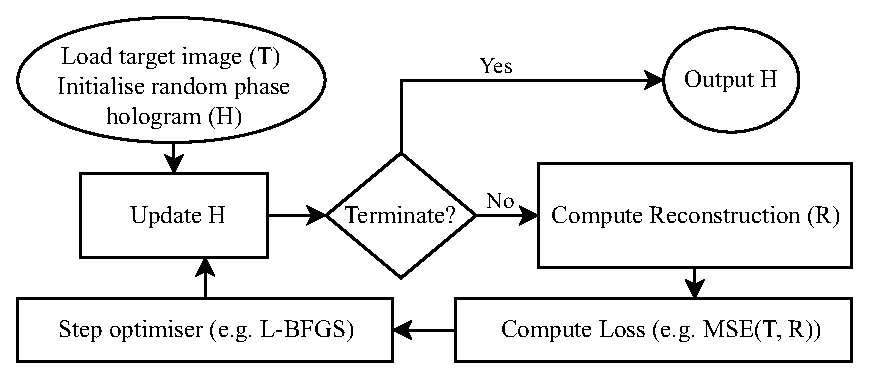
\includegraphics[width=\textwidth]{optim_flowchart_2D.eps}
	\caption{Flowchart of the optimisation process}
	\label{fig:optim_flowchart_2D}
\end{figure}

The optimisation process for generating a phase hologram to reconstruct a target image is depicted in \cref{fig:optim_flowchart_2D}. The process begins by loading the target image ($\textbf{T}$) and initializing a random phase hologram ($\textbf{H}$). Using this initial phase hologram, a reconstruction ($\textbf{R}$) of the target image is computed via either the Fraunhofer or Fresnel propagation equation introduced in \cref{sec:Diffraction} based on the distance needed. The difference between the target image ($\textbf{T}$) and the reconstruction ($\textbf{R}$) is quantified by computing the loss, such as the MSE in \cref{eq:MSE}. An optimiser (such as the GD, Adam or L-BFGS algorithms mentioned in \cref{sec:Numerical Optimisation Methods}) then updates the phase hologram based on the computed loss. This iterative process of reconstruction, loss calculation, and hologram update continues until a termination condition is met, usually a fixed total number of iterations, or when optimisation has reached convergence. The final optimised phase hologram ($\textbf{H}$) is then outputted.

\begin{figure}[H]
	\centering
	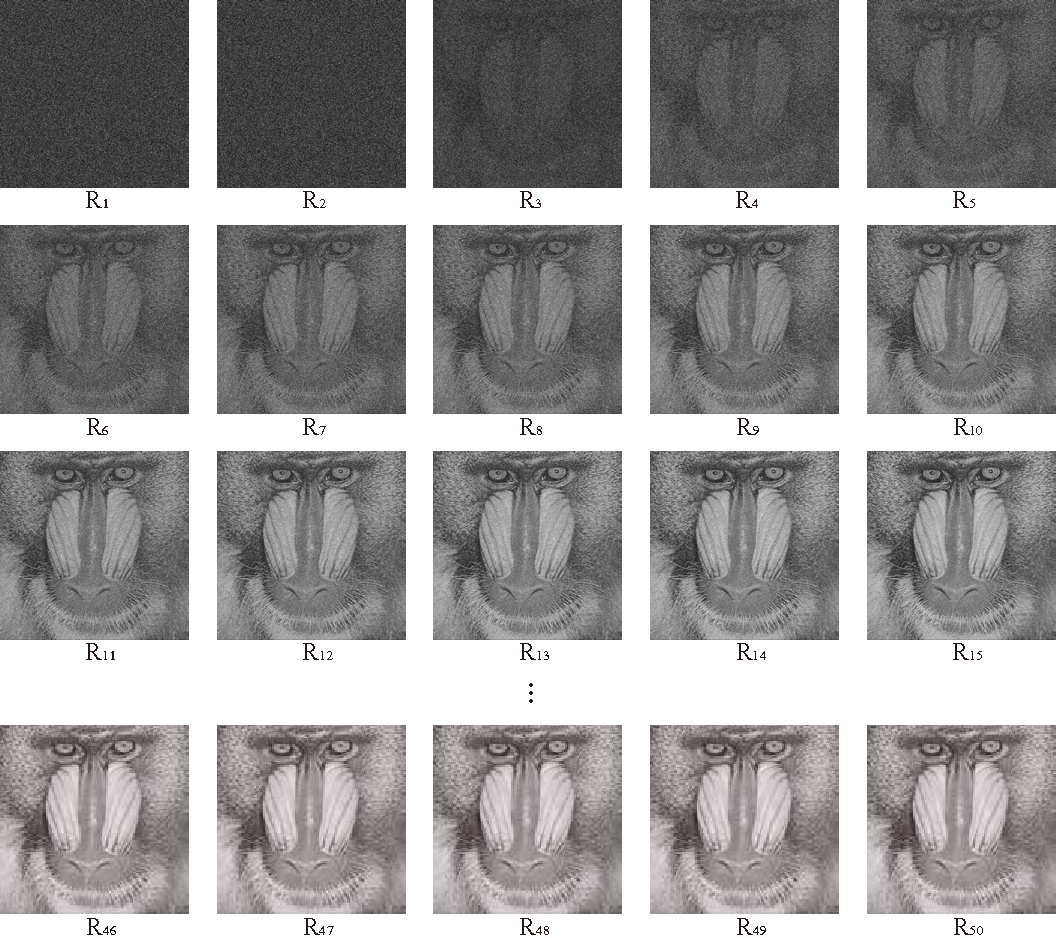
\includegraphics[width=\textwidth]{LBFGS_iters.pdf}
	\caption{Reconstructions at each iteration of the L-BFGS optimisation}
	\label{fig:LBFGS_iters}
\end{figure}

The optimisation flowchart in \cref{fig:optim_flowchart_2D} is run on the example target image in \cref{fig:mandrill.png} for a total of 50 iterations. The reconstruction ($\textbf{R}$) at each iteration is listed in \cref{fig:LBFGS_iters}, with iterations 16 to 45 omitted to save space. The list of reconstructions demonstrate visually how the optimisation converges to the resulting reconstruction ($\textbf{R}_{50}$) which has a very good quality. It shows that the proposed method using the L-BFGS algorithm to generate phase hologram is effective.

\begin{figure}[H]
	\centering
	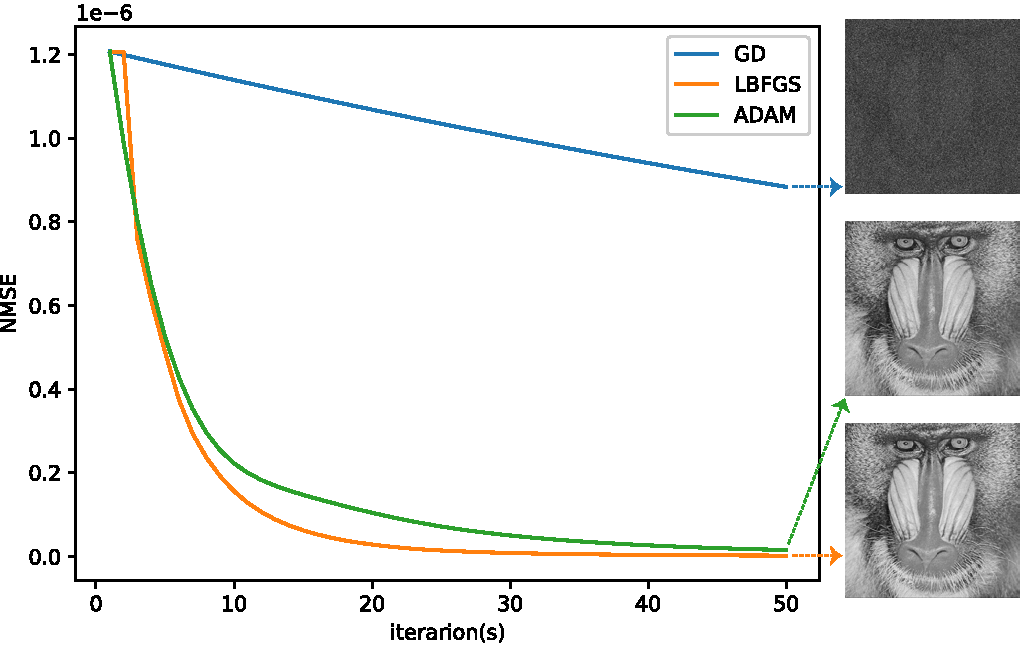
\includegraphics[width=\textwidth]{GD_ADAM_LBFGS.pdf}
	\caption{Convergence plot for comparison between the GD, Adam and L-BFGS optimisations}
	\label{fig:GD_ADAM_LBFGS}
\end{figure}

Then the proposed method of using L-BFGS algorithm to generate phase hologram is quantitatively compared against the existing methods using GD and Adam algorithms, by plotting the normalised mean-squared error (NMSE) which is simply the MSE in \cref{eq:MSE} divided by the sum of squares of the target image value, so that pixel values are normalised, avoiding the huge difference in MSE value which is based on how the value range is defined (typically 0-1 or 0-255).

The proposed method using L-BFGS algorithm (the yellow line in \cref{fig:GD_ADAM_LBFGS}) stagnates for the first two iterations as it needs to estimate the hessian as explained in \cref{sec:L-BFGS}. After the brief stagnation, the L-BFGS converges quickly, surpassing the existing methods in the literature using GD and Adam optimiser, corresponding to the blue line and the green line in \cref{fig:GD_ADAM_LBFGS} respectively. The final reconstructions are shown aside the NMSE plots, from which it can be seen that the L-BFGS algorithm produces a reconstruction of similar quality to the Adam algorithm, and both of them are much better than the GD algorithm. Such observation matches the final NMSE values. In summary, the L-BFGS algorithm was proven to be able to optimise a phase-only hologram for a target image, and is better than the Adam and GS optimisation algorithms.



\section{Target Image Phase Optimisation (TIPO)}
This section proposes a novel method of optimising the phase of the target image instead of optimising the phase of the hologram as previously introduced in \cref{sec:Optimisation of Phase Hologram for a Target Image}, under the same `phase only' constraint of the hologram. The objective is to find an optimal phase profile to be attached to the target image, so that its inverse propagation to the hologram plane produces a hologram whose phase has a reconstruction that best matches the target image. As it optimises the phase of the target image instead of the traditional way optimising the phase of the hologram, this method is named as Target Image Phase Optimisation (TIPO). A flowchart is drawn in \cref{fig:TIPO_flowchart} to clarify the detailed operation of the proposed TIPO algorithm.

\begin{figure}[H]
	\centering
	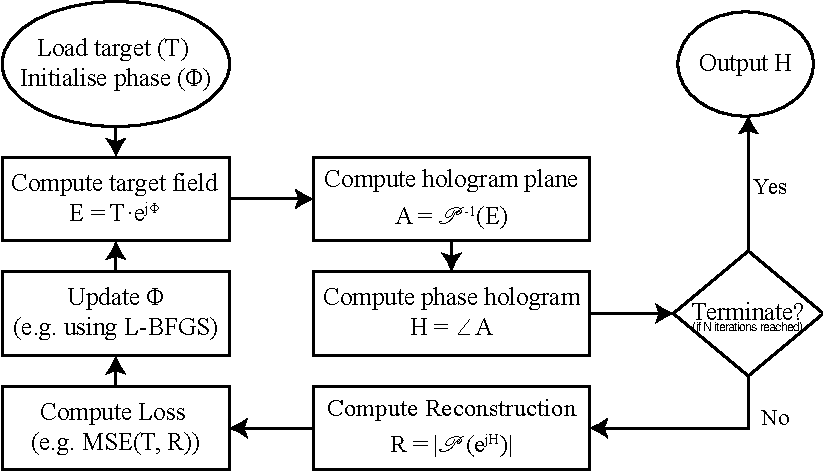
\includegraphics[width=\textwidth]{TIPO_flowchart.pdf}
	\caption{TIPO flowchart}
	\label{fig:TIPO_flowchart}
\end{figure}

The flowchart in \cref{fig:TIPO_flowchart} outlines the TIPO algorithm process for generating a phase-only hologram ($\textbf{H}$) to reconstruct a target image ($\textbf{T}$). The procedure starts with loading the target image and initializing the phase ($\Phi$). The complex target field ($\textbf{E}$) is then computed from the target image and the target image phase ($\textbf{E} = \textbf{T} \cdot e^{j\Phi}$). Next, the hologram aperture ($\textbf{A}$) is computed by applying the inverse propagation ($\mathcal{P}^{-1}$) to the target field, where $\mathcal{P}$ is chosen from the Fraunhofer and Fresnel diffraction equations in \cref{sec:Diffraction}. The phase-only hologram ($\textbf{H}$) is then derived from the angle of the complex hologram aperture ($\textbf{H} = \angle \textbf{A}$). Subsequently, a reconstruction ($\textbf{R}$) is computed using the forward propagation ($\textbf{R} = |\mathcal{P}(e^{jH})|$). The loss, such as the Mean Squared Error (MSE), is calculated between the target image ($\textbf{T}$) and the reconstruction ($\textbf{R}$). An optimiser (e.g. SGD or L-BFGS) then updates the phase ($\Phi$) based on the computed loss. This iterative process of computing the target field, hologram plane, phase hologram, reconstruction, and loss calculation continues, followed by phase updates, until a termination condition is met, which is usually set for a fixed number of iterations. Upon convergence, the final optimised phase hologram ($\textbf{H}$) is produced.

\begin{figure}[H]
	\centering
	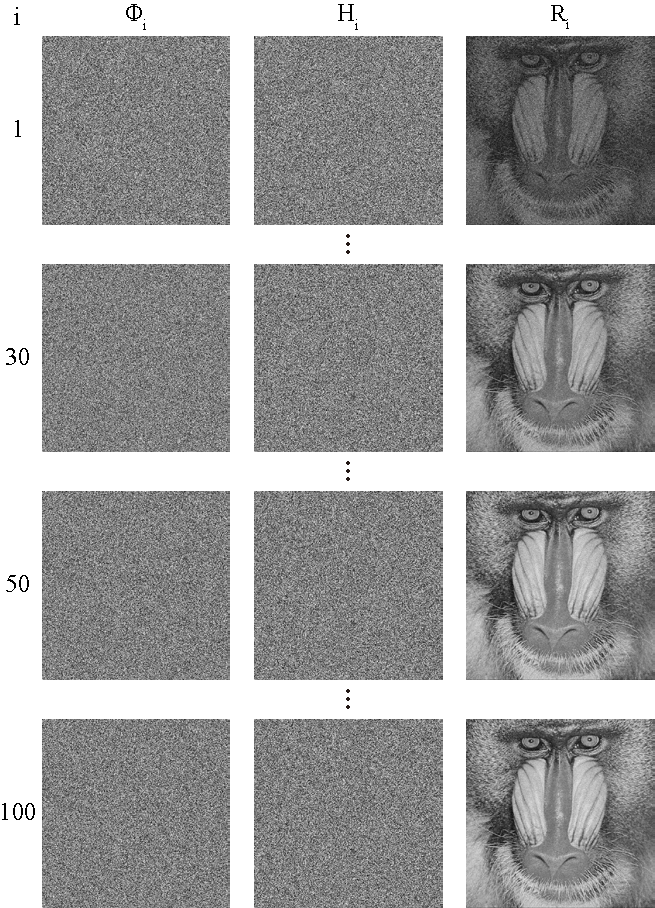
\includegraphics[width=0.8\textwidth]{TIPO_iters.pdf}
	\caption{TIPO iterations on the mandrill target}
	\label{fig:TIPO_iters}
\end{figure}

The results for an example run of the TIPO algorithm on the mandrill target (in \cref{fig:mandrill.png}) with the total number of iterations set to 100 are shown in \cref{fig:TIPO_iters} (only iterations number 1, 30, 50 and 100 are shown for space saving). As the first hologram is computed by the inverse propagation ($\mathcal{P}^{-1}$) of the target image with an random phase, the reconstruction ($\textbf{R}_1$) is already showing the target image. Then as the iterations continue, the reconstruction quality gets better, proving the effectiveness of the proposed TIPO algorithm.

\begin{figure}[H]
	\centering
	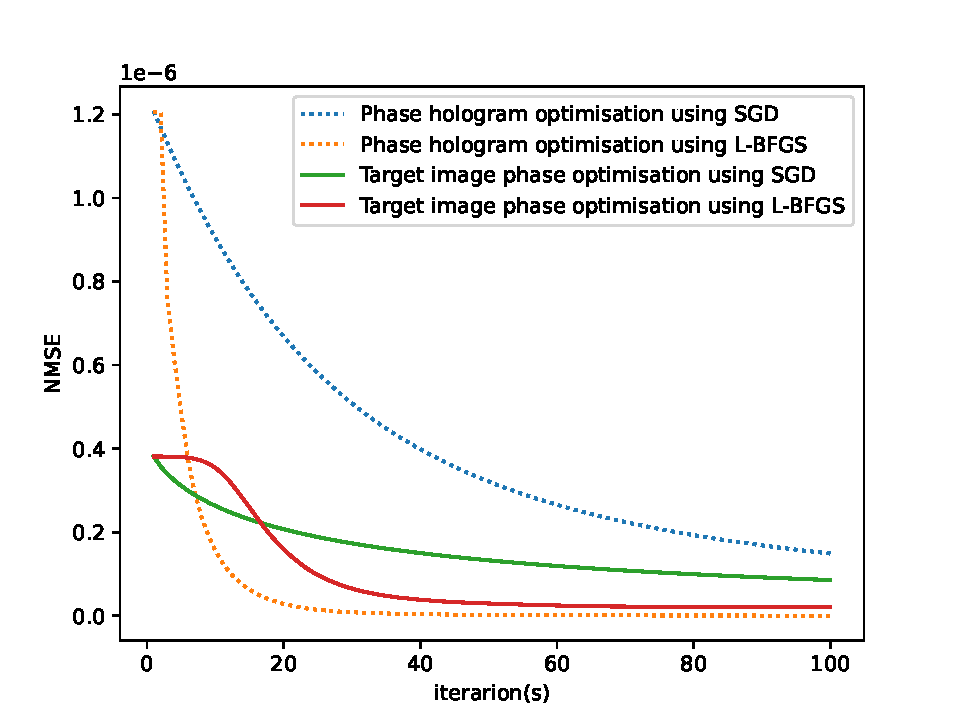
\includegraphics[width=\textwidth]{TIPO_convergence.pdf}
	\caption{TIPO convergence plot}
	\label{fig:TIPO_convergence}
\end{figure}

To quantitatively analyse the results, the convergence of the TIPO algorithm is plotted in \cref{fig:TIPO_convergence}, where the NMSE between the reconstruction and the target image are plotted against the number of iterations. Both SGD and L-BFGS optimisers are run for the TIPO algorithm (corresponding to the green and red line in \cref{fig:TIPO_convergence} accordingly), and are compared against the regular phase hologram optimisation algorithm in \cref{sec:Optimisation of Phase Hologram for a Target Image} (corresponding to the dotted blue line and the dotted yellow line in \cref{fig:TIPO_convergence} respectively). The TIPO algorithms using both SGD and L-BFGS optimisers start with a lower NMSE of the reconstruction as their holograms in the first iteration are extracted from the inverse propagation of the target image, instead of pure random holograms as done in the regular phase hologram optimisation. However, the regular phase hologram optimisation using L-BFGS optimiser quickly surpassed the TIPO algorithm within 10 iterations, and reached the lowest reconstruction error. For the SGD optimiser, the TIPO method (green line) has an significant improvement than the regular phase hologram optimisation method (dotted blue line). The two TIPO methods (in solid lines) lie between the two regular phase hologram optimisation method (in dotted lines), proving that although not being the best, the TIPO method is still an effective method for phase hologram generation.



\section{Multi-Depth Phase-Only Hologram Optimisation with Sequential Slicing}\label{sec:Multi-Depth Phase-Only Hologram Optimisation}

This chapter implements the limited-memory Broyden-Fletcher-Goldfarb-Shanno (L-BFGS) optimisation method to generate phase-only computer-generated hologram (CGH) for 3D targets. In addition to reviewing the existing multi-depth hologram optimisation methods which computes the full 3D reconstruction of the hologram at every iteration, this chapter proposes a novel method called sequential slicing (SS) for a partial evaluation of the hologram during each optimisation iteration.

\subsection{Introduction}
A search in the literature has found some recent work that compute CGH for 3D targets using numerical optimisation methods \cite{Zhang2017, Liu2020, Choi2021, Chen2021}, but speed and quality are still the major challenges. They either evaluate the error of reconstructions against the entire 3D target, which is time-consuming, or evaluate the hologram for each plane and then sum the holograms, which introduces quality degradation.

This chapter proposes the sequential slicing (SS) technique for the L-BFGS optimisation of CGH for multi-depth 3D target, which evaluates the loss for a single slice at each iteration. The proposed technique aims for a quicker hologram generation with proper overall quality and low quality imbalance across the multiple depths, benefiting from the second-order nature of the L-BFGS optimiser.


\subsection{Methods}

The optimiser used for CGH in this chapter is the L-BFGS optimiser as introduced in \cref{sec:L-BFGS}, with the GD optimiser in \cref{sec:GD} also implemented as a reference. The phase-only constraint of CGH is applied by fixing a constant amplitude of the hologram, while keeping its phase varying and being the argument of optimisation ($\textbf{x}$ in \cref{eq:minimise_F}).

\begin{figure}[H]
	\centering
	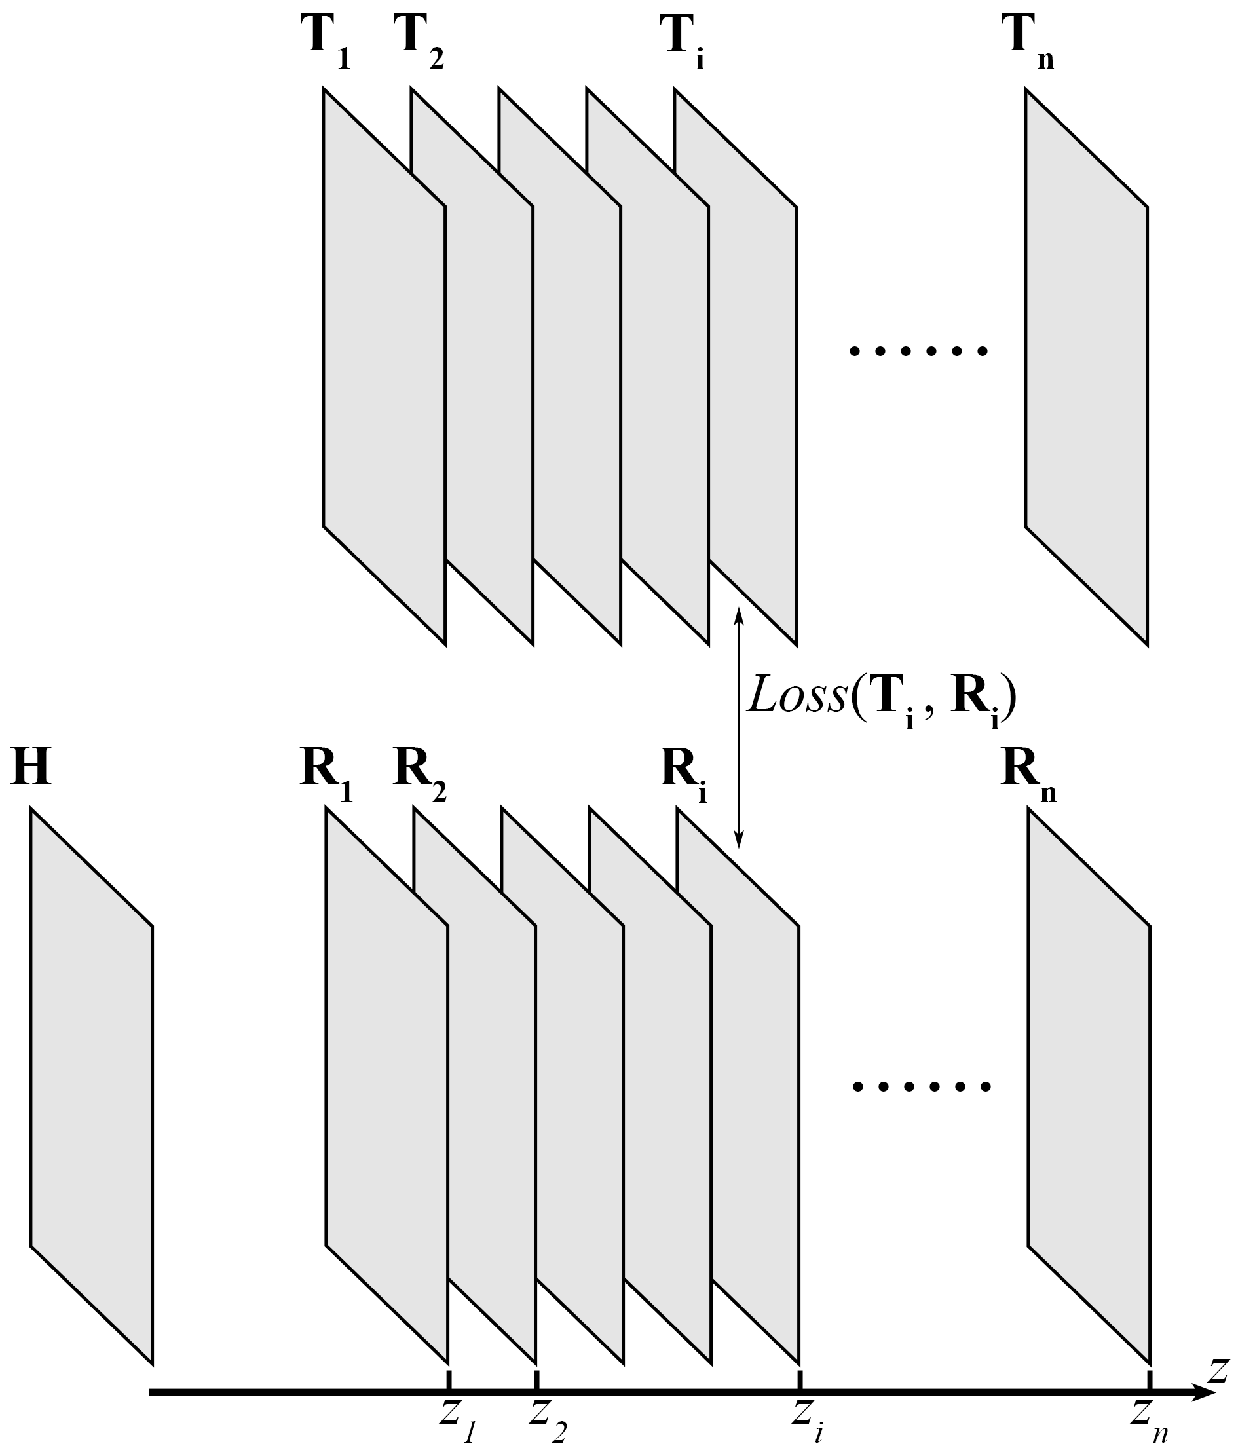
\includegraphics[width=0.6\textwidth]{Fresnel_slice_illustration}
	\caption{Loss between the multi-depth targets ($\textbf{T}_1$ to $\textbf{T}_n$) and the reconstructions ($\textbf{R}_1$ to $\textbf{R}_n$) of hologram $\textbf{H}$}
	\label{fig:Fresnel_slice_illustration}
\end{figure}

As shown in \cref{fig:Fresnel_slice_illustration}, the multi-depth target is set up as a collection of $n$ slices ($\textbf{T}_1$ to $\textbf{T}_n$), each slice $\textbf{T}_i$ is at a distance $z_i$ to the hologram plane. And for the hologram $\textbf{H}$, its reconstruction at each distance $z_i$ is computed using Fresnel diffraction formula in \cref{eq:fresnel-diffraction}, which is labelled as the propagation function $\mathcal{P}(\textbf{H}, z_i)$.

\subsubsection{Loss Functions}
To formulate an objective function $f(\textbf{x})$ in \cref{eq:minimise_F}, we need to quantify the difference between each target slice ($\textbf{T}_i$) and the respective reconstruction ($\textbf{R}_i$) numerically, which is denoted as $Loss(\textbf{T}_i, \textbf{R}_i)$ in \cref{fig:Fresnel_slice_illustration}. In addition to the mean squared error (MSE) \cite{MSE_REF} previously used in \cref{sec:Optimisation of Phase Hologram for a Target Image}, the cross entropy (CE) \cite{cybenko1998mathematics} and relative entropy (RE) \cite{Kullback1951} are also implemented. To adapt the loss functions for two-dimensional (2D) target image $\textbf{T}_i$ and reconstructed image $\textbf{R}_i$ of dimension $X\times Y$, the loss functions are adapted as shown in \cref{eq:MSE_holo} to \cref{eq:RE_holo}.

\begin{align}
	MSE(\textbf{T}_i, \textbf{R}_i) & = \frac{1}{X\times Y} \sum_{x=1}^{X} \sum_{y=1}^{Y} (\textbf{T}_{i;x,y}-\textbf{R}_{i;x,y})^2\label{eq:MSE_holo}                     \\
	CE(\textbf{T}_i, \textbf{R}_i)  & = -\sum_{x=1}^{X} \sum_{y=1}^{Y} \textbf{T}_{i;x,y}\log(\textbf{R}_{i;x,y})\label{eq:CE_holo}                                        \\
	RE(\textbf{T}_i, \textbf{R}_i)  & = -\sum_{x=1}^{X} \sum_{y=1}^{Y} \textbf{T}_{i;x,y}\log\left(\frac{\textbf{R}_{i;x,y}}{\textbf{T}_{i;x,y}}\right) \label{eq:RE_holo}
\end{align}

MSE is a traditional metric averaging the squared error between the target and observed values. CE, adapted as shown in \cref{eq:CE_holo}, is usually used in classification problems, such as language modelling \cite{Liu2018}. RE, also called Kullback-Leibler divergence (usually denoted as $D_{KL}(P\vert\vert Q)$, but is denoted as RE here for uniformity), is adapted as shown in \cref{eq:RE_holo}. RE is usually used to measure how much a probability distribution $P$ is different from another probability distribution $Q$. Both CE and RE are usually computed between the true probabilistic distribution and the predicted probabilistic distribution. While the images are not probability distributions, the pixel values can be normalized to decimal numbers in the range from 0 to 1 so that CE and RE can be applied.

\subsubsection{Optimisation Techniques}
\paragraph{Sum-of-Loss (SoL) technique}
The conventional technique to compute 3D CGH is to sum the losses for each slice at each iteration during optimisation, which is called the Sum-of-Loss (SoL) method here. At every iteration, it computes the full 3D reconstructions ($\textbf{R}_1, \cdots, \textbf{R}_n$) of the hologram $\textbf{H}$ at every distance $z_i$, and then sum the losses between each pair of reconstruction $\textbf{R}_i$ and target image $\textbf{T}_i$. The mathematical expression of the SoL technique's optimisation objective is shown below:
\begin{equation}
	\text{SoL:}\quad \underset{\textbf{H}}{\arg \min}\ \sum_{i = 1}^{n} Loss(\textbf{T}_i, \textbf{R}_i)
\end{equation}

The SoL method requires a total of $n$ Fourier Transforms to fully evaluate the hologram at each step, making it computationally heavy.

\paragraph{Sum-of-Hologram (SoH) technique}
Another technique for 3D CGH is to compute the complex sum of the sub-holograms $\textbf{H}_i$ generated for each target slice $\textbf{T}_i$ to form a total hologram based on the principle of superposition, which is called the Sum-of-Hologram (SoH) method here. The SoH technique's mathematical expression is shown in \cref{eq:SoH} below:
\begin{equation}
	\text{SoH:}\quad \angle \sum_{i = 1}^{n} e^{j \cdot \underset{\textbf{H}_i}{\arg \min}\ Loss(\textbf{T}_i, \textbf{R}_i)}
	\label{eq:SoH}
\end{equation}

The sub-hologram $\textbf{H}_i$ for each slice number $i$ is computed independently with the optimisation objective of $\underset{\textbf{H}_i}{\min}\ Loss(\textbf{T}_i, \textbf{R}_i)$, the arguments of which are then summed in a complex manner, as each phase hologram is the angle, the exponential operator is needed to turn angles into complex numbers. Lastly, the angle of the complex sum is taken so that it can meet the `phase-only' constraint.

If using a fixed number of iterations per sub-hologram, the total computation scales up linearly with the number of slices $n$. The SoH method's advantage is its ease of implementation, that any existing single slice CGH algorithm can be quickly converted to multi-depth 3D CGH algorithm. Its major disadvantage for phase-only hologram generation is that, the final summing of sub-holograms will result in a non-uniform amplitude hologram, and taking the phase of which will result in discarding the amplitude information of the summed hologram, leading to deprecations in reconstructions quality. And also, the SoH method suffers from the defocusing effect between the each slice to another, causing additional noise.

\paragraph{Sequential Slicing (SS) technique}
\begin{figure}[H]
	\centering
	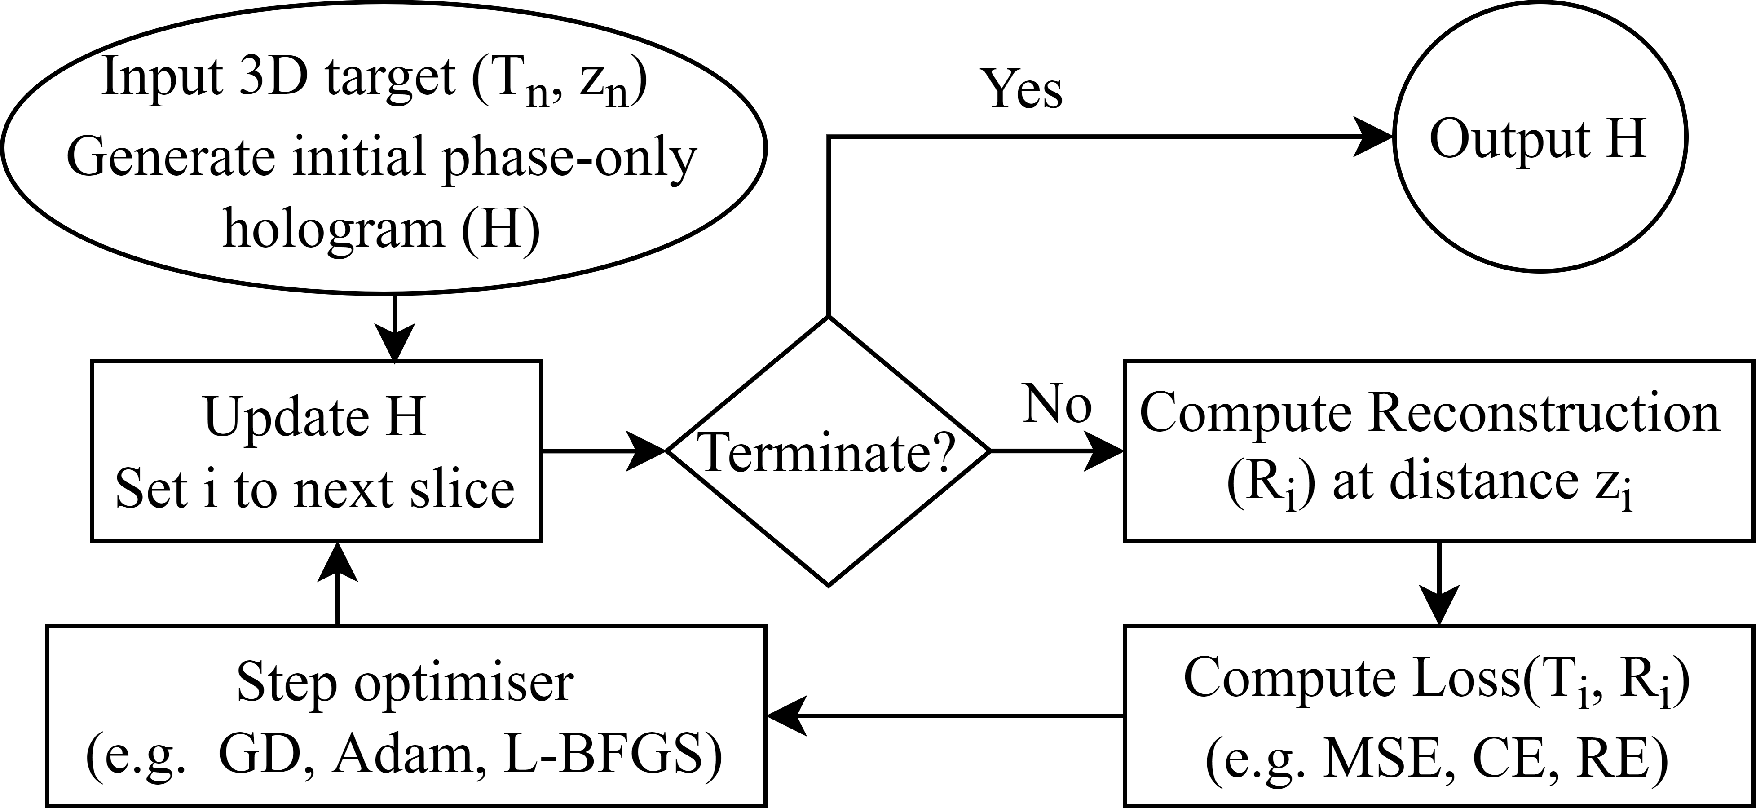
\includegraphics[width=0.8\textwidth]{optim3d-cgh-flowchart}
	\caption{Optimisation of CGH with sequential slicing (SS) flowchart}
	\label{fig:optim3d-cgh-flowchart}
\end{figure}

This section proposes the novel CGH optimisation with sequential slicing (SS) technique, as shown in the flowchart in \cref{fig:optim3d-cgh-flowchart}, that only computes the loss for a single slice at each iteration (between a reconstruction $\textbf{R}_i$ at a single distance $z_i$ and its according target slice $\textbf{T}_i$), where $i$ sweeps through the multi-layer 3D target sequentially when the algorithm iterates. When the final slice is reached ($i=n$), it goes back to the first slice ($i \gets 1$). The proposed method only needs to carry out one Fourier Transform at each iteration, and the number of iterations does not need to scale up with $n$. So it is expected to be much quicker than SoL and SoH techniques while producing proper resulting hologram.








%%%%%%%%%%%%%%%%%%%%%%%%%%  Results  %%%%%%%%%%%%%%%%%%%%%%%%%%
\subsection{Results}
\subsubsection{CGH for a 4-slice target}

\begin{figure}[H]
	\centering
	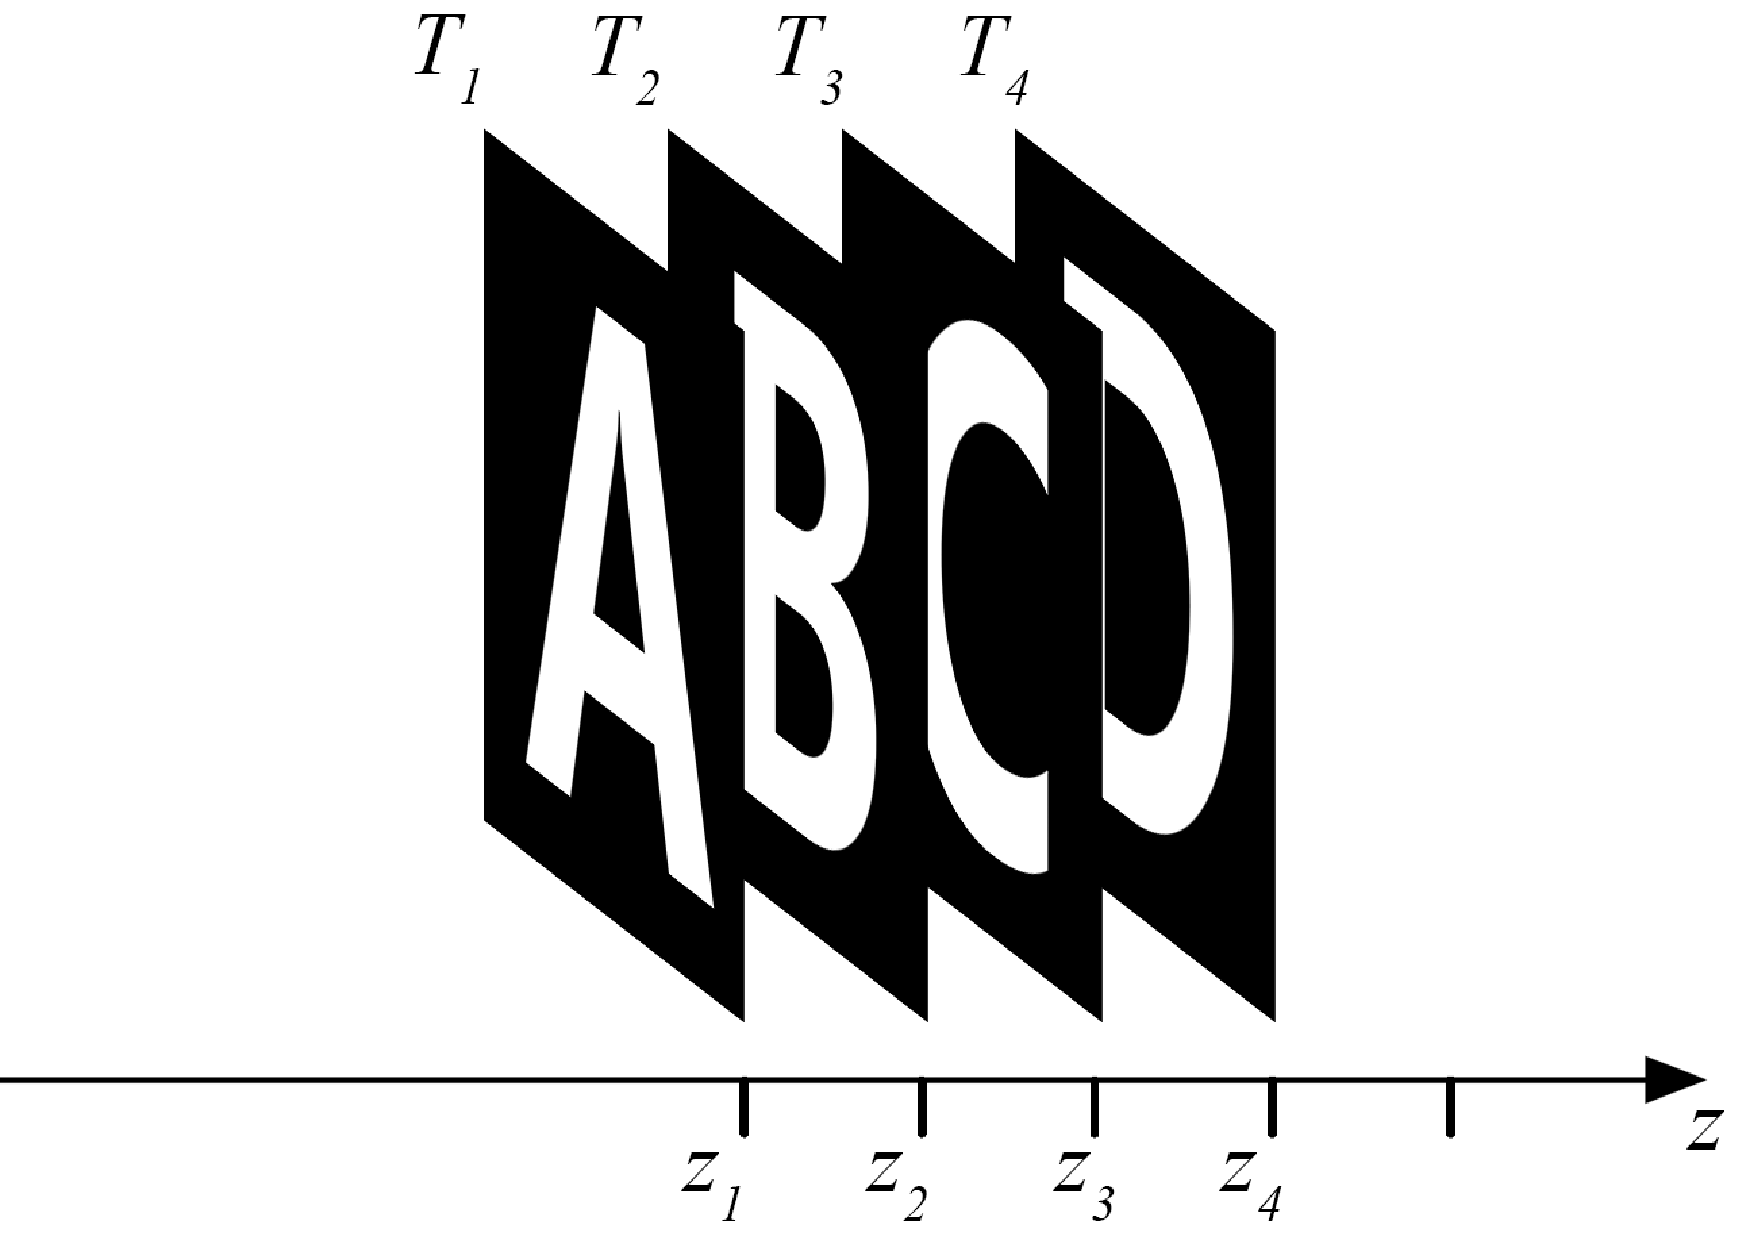
\includegraphics[width=0.7\textwidth]{Fresnel_slice_ABCD}
	\caption{Layout of the 4-slice target ($z_1=1\ cm$, $z_2=2\ cm$, $z_3=3\ cm$, $z_4=4\ cm$)}
	\label{fig:Fresnel_slice_ABCD}
\end{figure}

The first example 3D target used is consisted of 4 slices made from alphabets `A', `B', `C', `D', each having $512\times512$ pixels. The positions of the four slices range from $1\ cm$ to $4\ cm$ with $1\ cm$ gap between each other (i.e. $z_i=i\ cm$). The overall layout is shown in \cref{fig:Fresnel_slice_ABCD}.

As there are two optimisers (GD and L-BFGS), three techniques (SoL, SoH and SS) and three loss functions (MSE, CE, RE) in consideration, they can form a total of 18 combinations. In order to control the number of variables, all 18 combinations are set to start from the same initial random hologram and run for the same amount of 100 iterations for the optimisation of each hologram, on the same laptop of model ASUS ROG Zephyrus M16, which has a CPU of model i7-11800H and a GPU of model RTX3060. For the L-BFGS algorithm, the gradient history of size 10 ($m=10$ in \cref{alg:L-BFGS}) is used for all techniques and loss functions. And to ensure a sensible comparison, although three different loss functions are used for optimisation of CGH, the metric used to assess the final quality of multi-depth reconstructions of the hologram is the normalized mean squared error (NMSE). As there are a total of 4 slices in this example, the final NMSE of each are computed separately and the total optimisation run time is recorded. The final results are gathered in \cref{fig:Technique_Loss_comparison}. As each slice has a different final error, their mean and standard deviation (SD) are also computed for investigations. Three columns are colour coded where green indicates better result while red indicates worse result.

\begin{figure}[H]
	\centering
	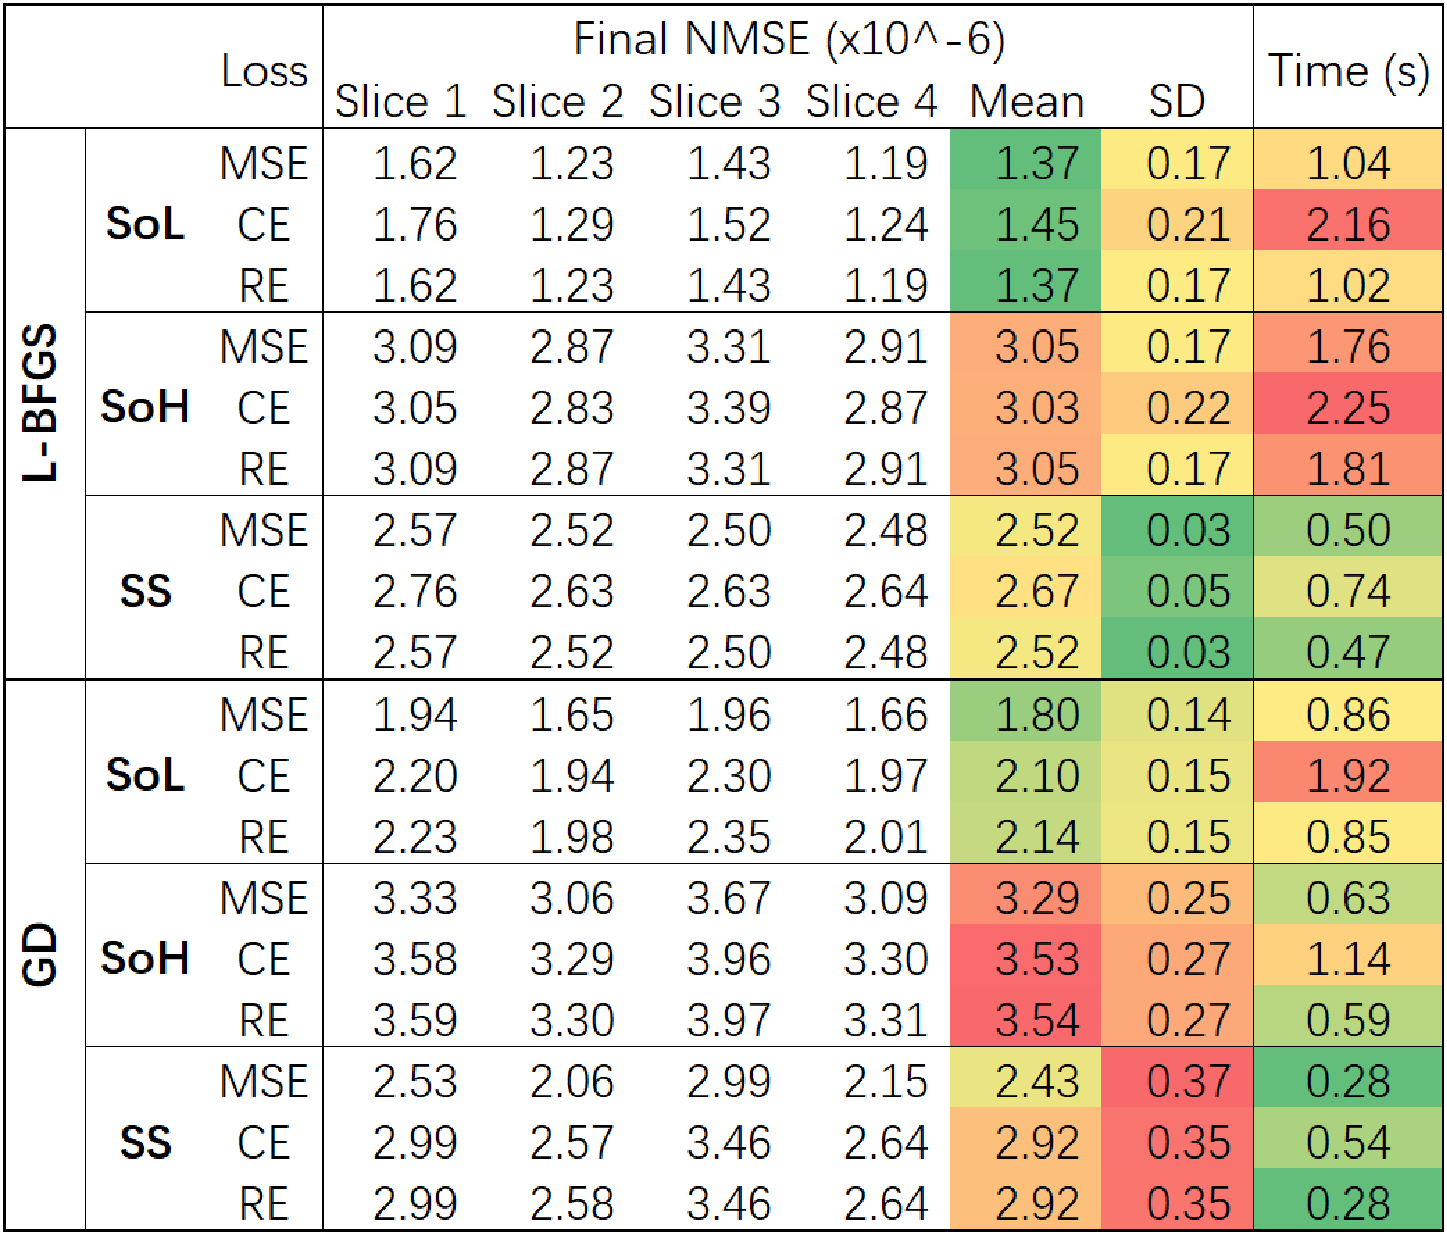
\includegraphics[width=0.8\textwidth]{Technique_Loss_comparison}
	\caption{Final NMSE and run time comparison across the three techniques}
	\label{fig:Technique_Loss_comparison}
\end{figure}

Comparing the mean of final NMSE and the run time of the proposed sequential slicing (SS) technique to those of the sum-of-loss (SoL) and sum-of-hologram (SoH) techniques in \cref{fig:Technique_Loss_comparison}, it can be concluded that, for all combinations of optimisers and loss functions attempted, the proposed SS technique runs much quicker than the existing SoL and SoH techniques, while still providing a proper result, sitting between the SoL and SoH techniques. So the SS technique has not demonstrated absolute advantage to the SoL technique yet on this 4-slice example, therefore further investigation will be done on a 30-slice example in \cref{sec:30-slice-target}.The SS technique is both quicker and has better reconstructions quality than the SoH technique, demonstrating an absolute advantage. Meanwhile, the runs with CE as loss function are much slower and has not demonstrated any advantage in the final NMSE, demonstrating an absolute disadvantage, so the results with CE loss or SoH method will not be shown in the per-iteration plots later in \cref{fig:SS_NMSE_iteration_compare}.

\begin{figure}[H]
	\centering
	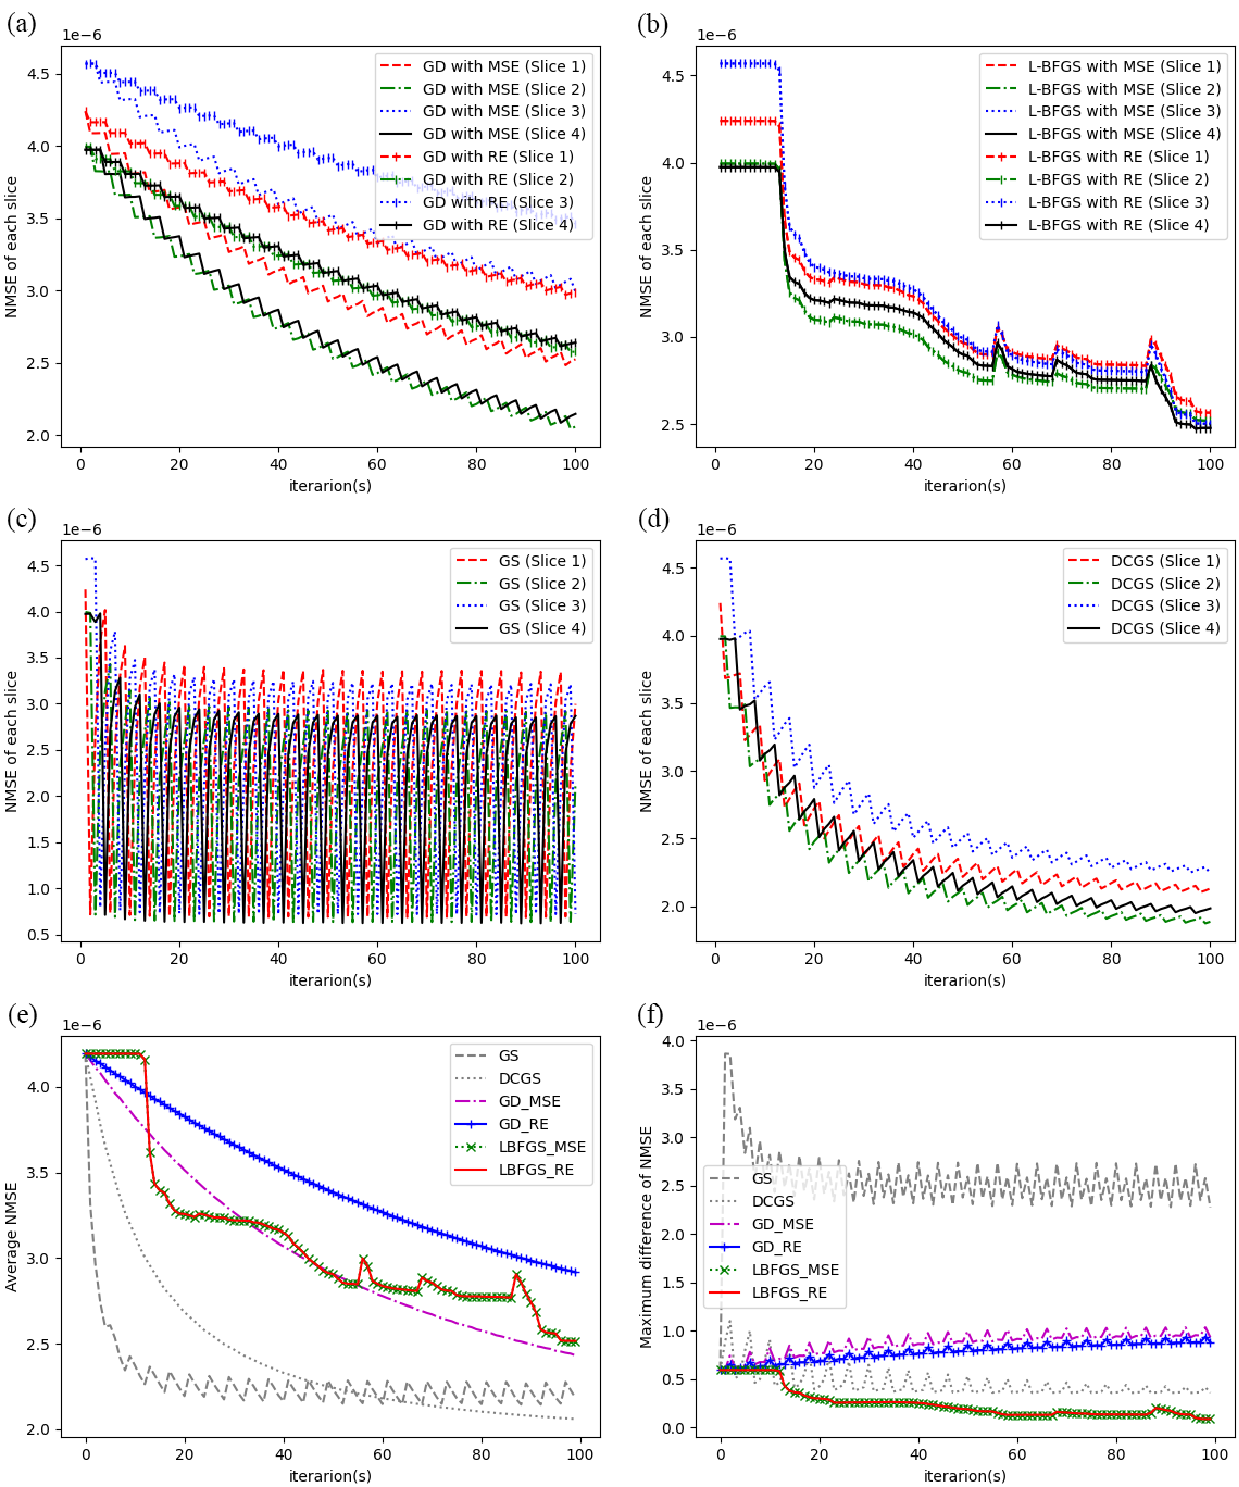
\includegraphics[width=1.0\textwidth]{Comparison_among_SS_methods_for_the_4_slice_target}
	\caption{Comparison among SS techniques for the 4-slice target using (a) GD algorithm, (b) L-BFGS algorithm, (c) GS algorithm, (d) DCGS algorithm. (e) Average NMSE, and (f) difference between the maximum and minimum NMSE across all slices.}
	\label{fig:SS_NMSE_iteration_compare}
\end{figure}
For comparison among the runs using the sequential slicing (SS) techniques, the NMSE for each slice and their average and maximum difference values are plotted for GD and LBFGS algorithms with MSE and RE loss functions in \cref{fig:SS_NMSE_iteration_compare}, and the GS-based sequential GS and DCGS \cite{Zhou2019} methods (mentioned in \cref{sec:GS algorithm adaptation}) are also implemented and plotted for reference purpose. For the plots of NMSE of each slice against iterations numbers in (\cref{fig:SS_NMSE_iteration_compare} (a, b, c, d)), apart from the L-BFGS algorithm, all the other algorithms (in \cref{fig:SS_NMSE_iteration_compare} (a, c, d)) are showing a staircase-like trend, where a decrease in error on one slice results in an increase in error on all other slices, and the final NMSE of each slice distinguishes a lot from another. The sequential GS algorithm suffers the most from the quality imbalance between each slice, and the sequential GD algorithm follows. The DCGS algorithm benefits from its modification of the inclusion of a weighting factor consisting historical amplitude, therefore managed to converge. From the average NMSE plot (\cref{fig:SS_NMSE_iteration_compare} (e)), the proposed sequential L-BFGS method does not appear to have the lowest average NMSE, but it has the lowest quality imbalance across the slices as shown in the maximum difference plot (\cref{fig:SS_NMSE_iteration_compare} (f)). The L-BFGS algorithm mainly benefits from its inclusion of curvature information during optimisation, so that the update of hologram $\textbf{H}$ at each iteration takes into account not only the loss for current slice, but also all historical iterations up to the set history size ($m$ in \cref{alg:L-BFGS}). So the NMSE of each slice stays close for L-BFGS and at each iteration, the NMSE of all slices behave in the same way, ensuring each slice to have the similar quality. Therefore, the proposed SS technique with L-BFGS optimiser is shown to have the lowest quality imbalance across all slices.


\begin{figure}[H]
	\centering
	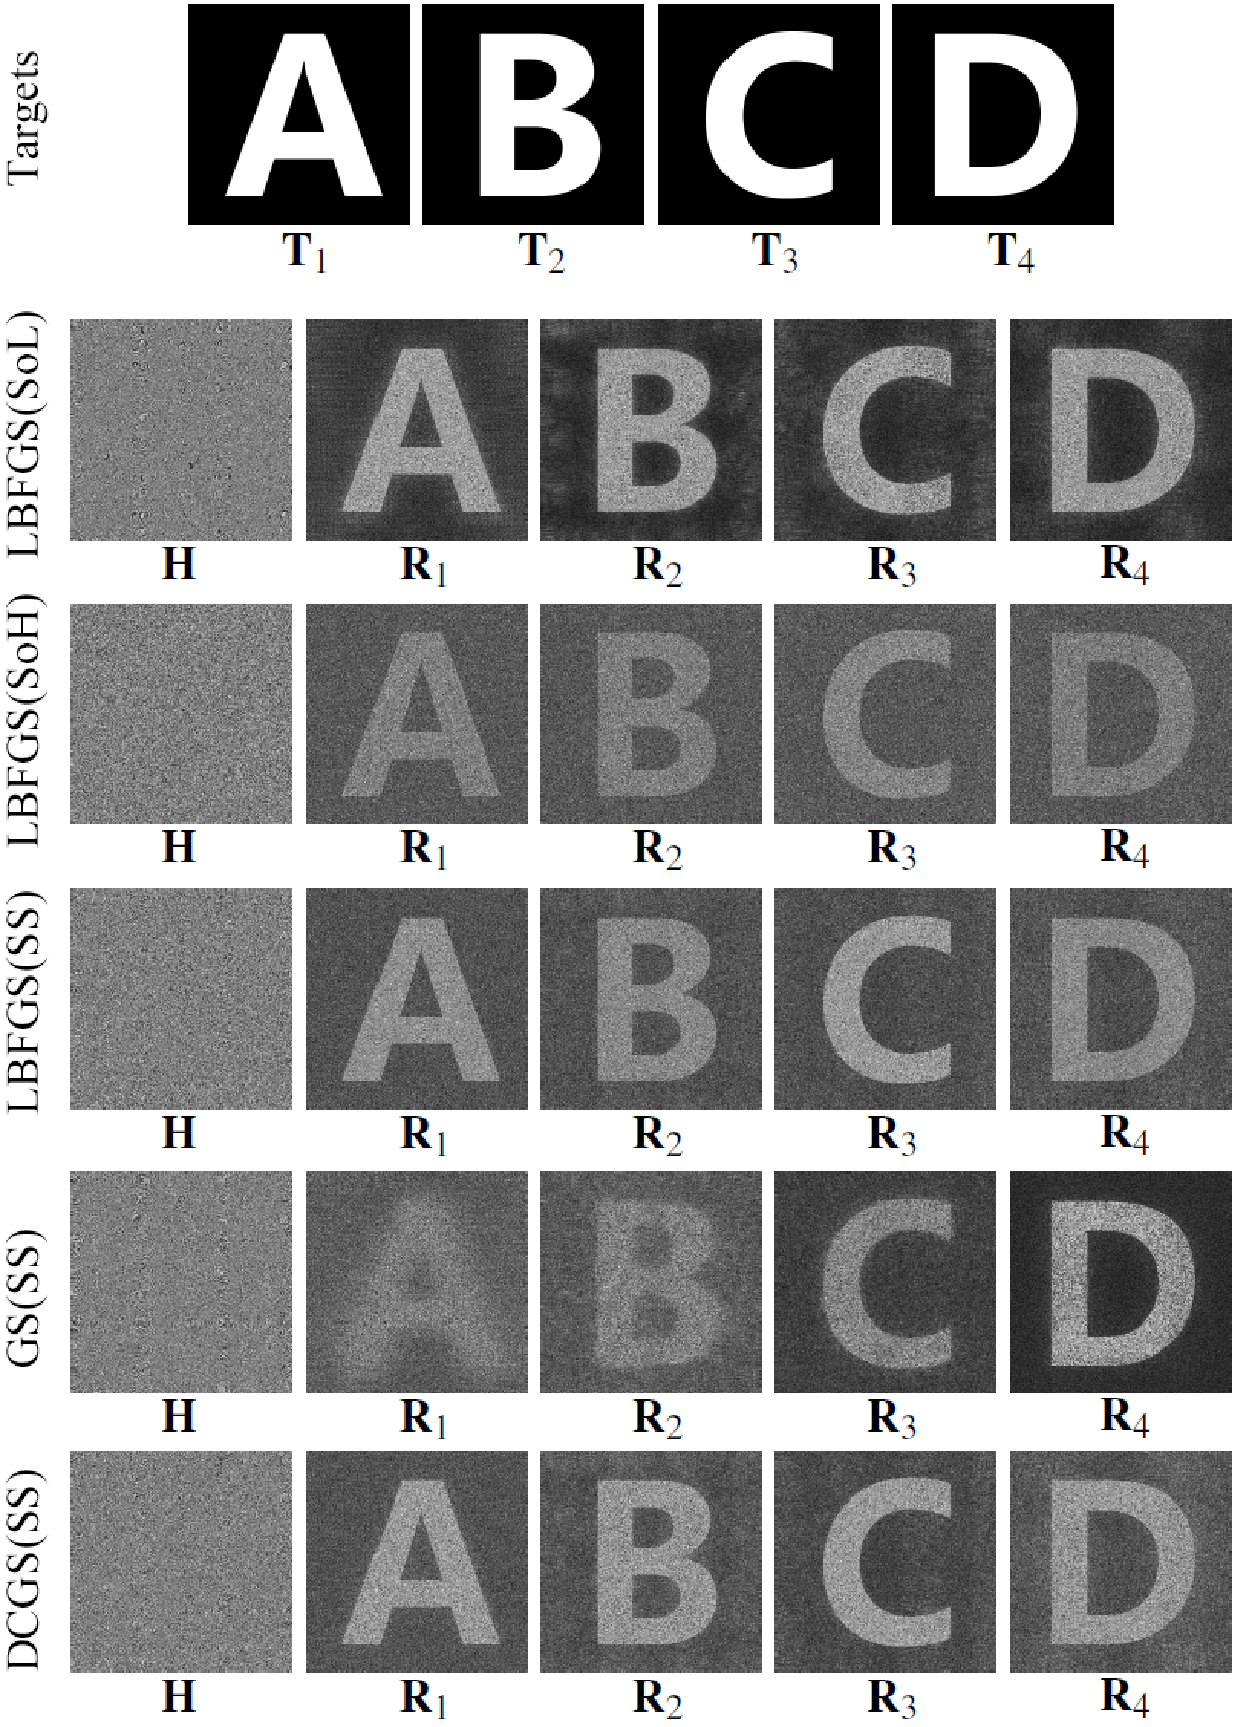
\includegraphics[width=0.7\textwidth]{final_holograms_reconstructions_4_slice}
	\caption{Comparison of final holograms and reconstructions}
	\label{fig:3D_ABCD}
\end{figure}

The final holograms and their reconstructions for L-BFGS algorithm with SoL, SoH and SS techniques are shown in \cref{fig:3D_ABCD}, with GS with SS technique and DCGS also shown as reference. The reconstructed images confirm the SS technique having a quality between SoH and SoL method (for the same amount of iterations), and has a much better quality imbalance than sequential GS, which has a very clear reconstruction at the fourth slice (letter `D') because the iteration stopped at the fourth slice but much worse reconstructions at other slices. Admittedly, the proposed L-BFGS with SS method cannot surpass the GS-based DCGS algorithm yet, but within the optimisation based algorithms, the proposed method has shown its advantage among the others.




\begin{figure}[H]
	\centering
	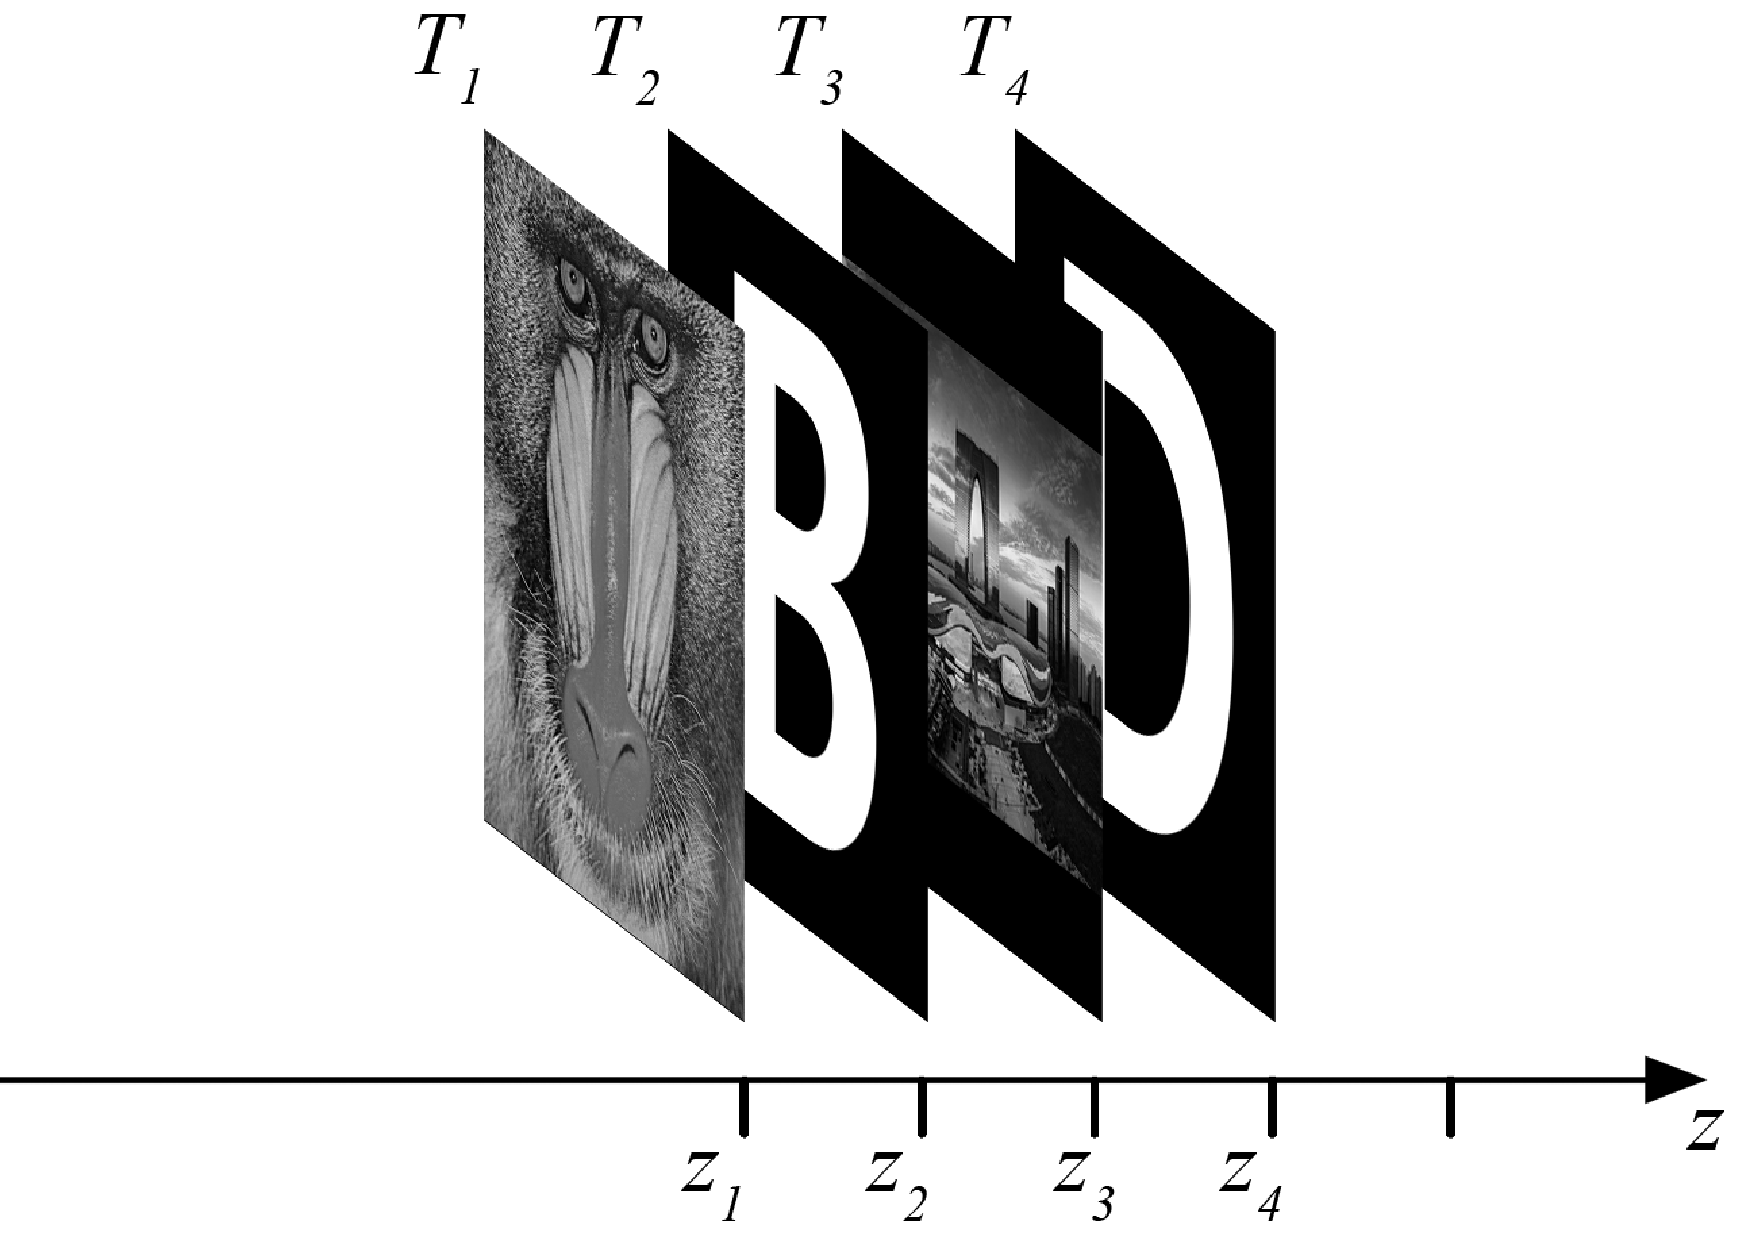
\includegraphics[width=0.7\textwidth]{Fresnel_slice_mandrill_B_szzx_D}
	\caption{Layout of the non-binary 4-slice target}
	\label{fig:more_difficult_3d_target_layout}
\end{figure}

To prove that the proposed method also works for non-binary valued target images, another example of a 4-slice 3D target is attempted, as shown in \cref{fig:more_difficult_3d_target_layout}, where two of the slices are replaced by an image of the mandrill \cite{MANDRILL_REF} and an image of the city scene \cite{Zhang2017} respectively.

\begin{figure}[H]
	\centering
	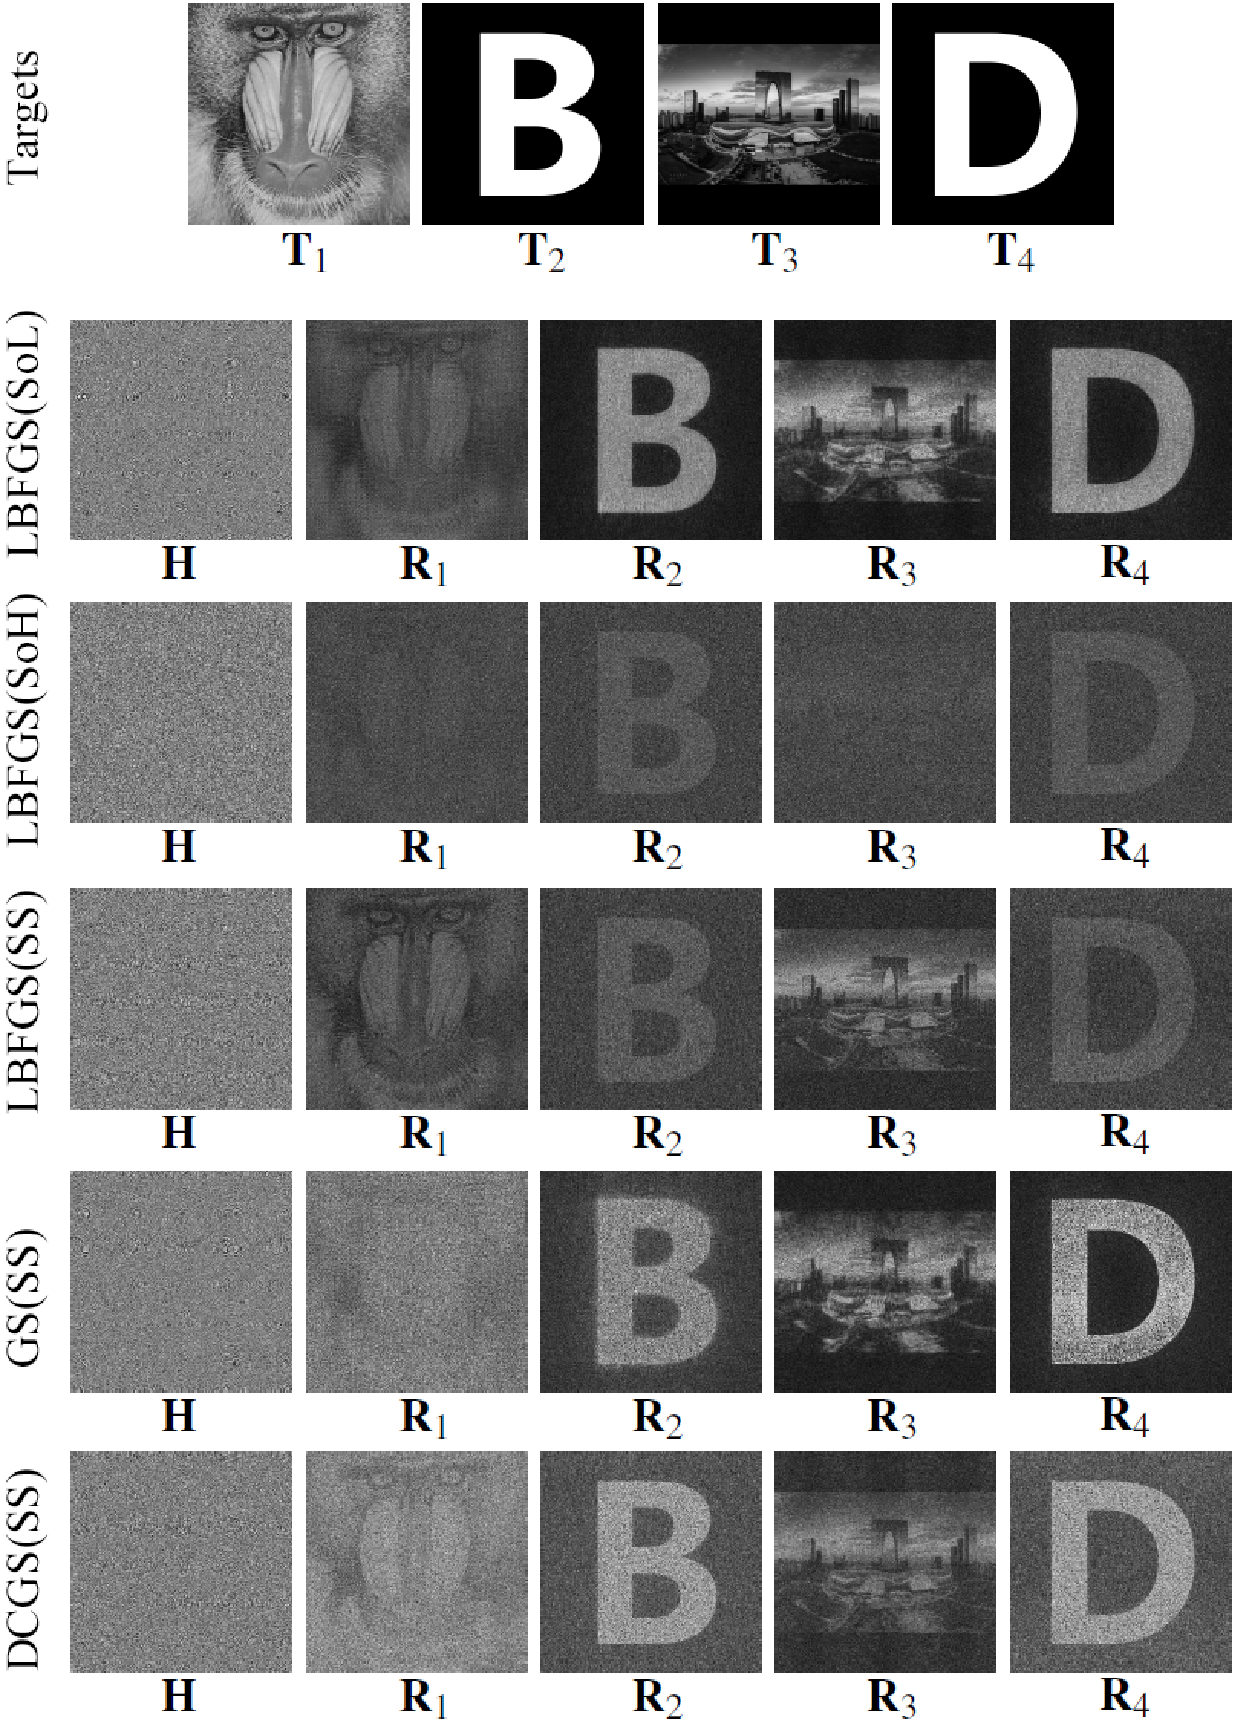
\includegraphics[width=0.7\textwidth]{final_holograms_reconstructions_4_slice_non_binary}
	\caption{Comparison of final holograms and reconstructions for non-binary target}
	\label{fig:more_difficult_3d_target_recon}
\end{figure}

As shown in the final holograms and reconstructions in \cref{fig:more_difficult_3d_target_recon}, the proposed LBFGS with SS technique still managed to converge, with final reconstructions quality sitting between the SoL and the SoH method, and also having a good quality balance across all slices. As the SS technique is faster than both the SoL and the SoH method, its quality performance is impressive.



\newpage
\subsubsection{CGH for a 30-Slice Target} \label{sec:30-slice-target}

\begin{figure}[H]
	\centering
	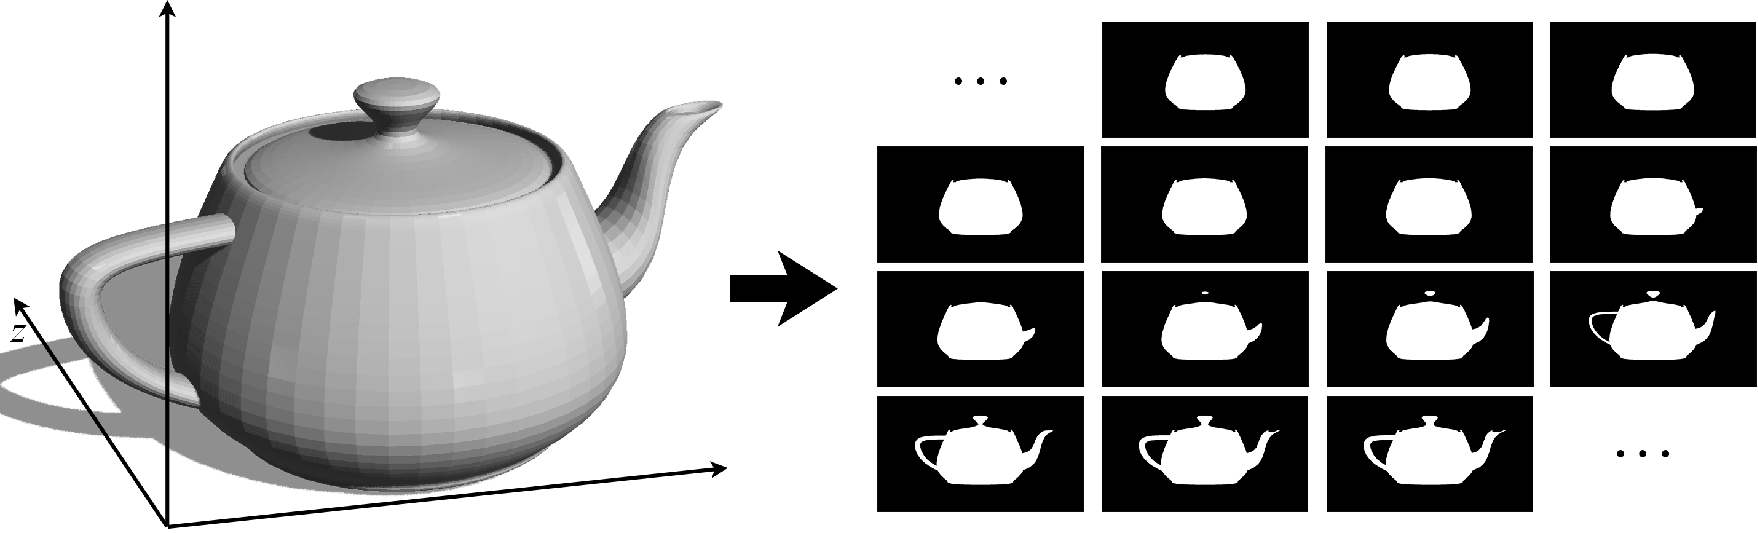
\includegraphics[width=1.0\textwidth]{Utah_teapot_target}
	\caption{30-slice target sliced from a 3D Teapot mesh}
	\label{fig:Teapot_target}
\end{figure}

Another example of a 30-slice target sliced from a 3D teapot is attempted for speed analysis when the number of slices go higher. As shown in \cref{fig:Teapot_target}, the Utah teapot \cite{Clark2015} is sliced into 30 planes, each of 720p resolution ($1280px\times720px$). Each combination in \cref{fig:Technique_Loss_comparison} were run on a laptop of model ASUS ROG Zephyrus M16 with a CPU of model i7-11800H and a GPU of model RTX3060. The average and maximum difference of NMSE across all slices plotted against time (in \cref{fig:Teapot_Average_NMSE_vs_time} and \cref{fig:Teapot_Max_diff_NMSE_vs_time} respectively) for all combinations except those with SoH technique or with CE loss function (as they are proven to have an absolute disadvantage), for clearer plots.

\begin{figure}[H]
	\centering
	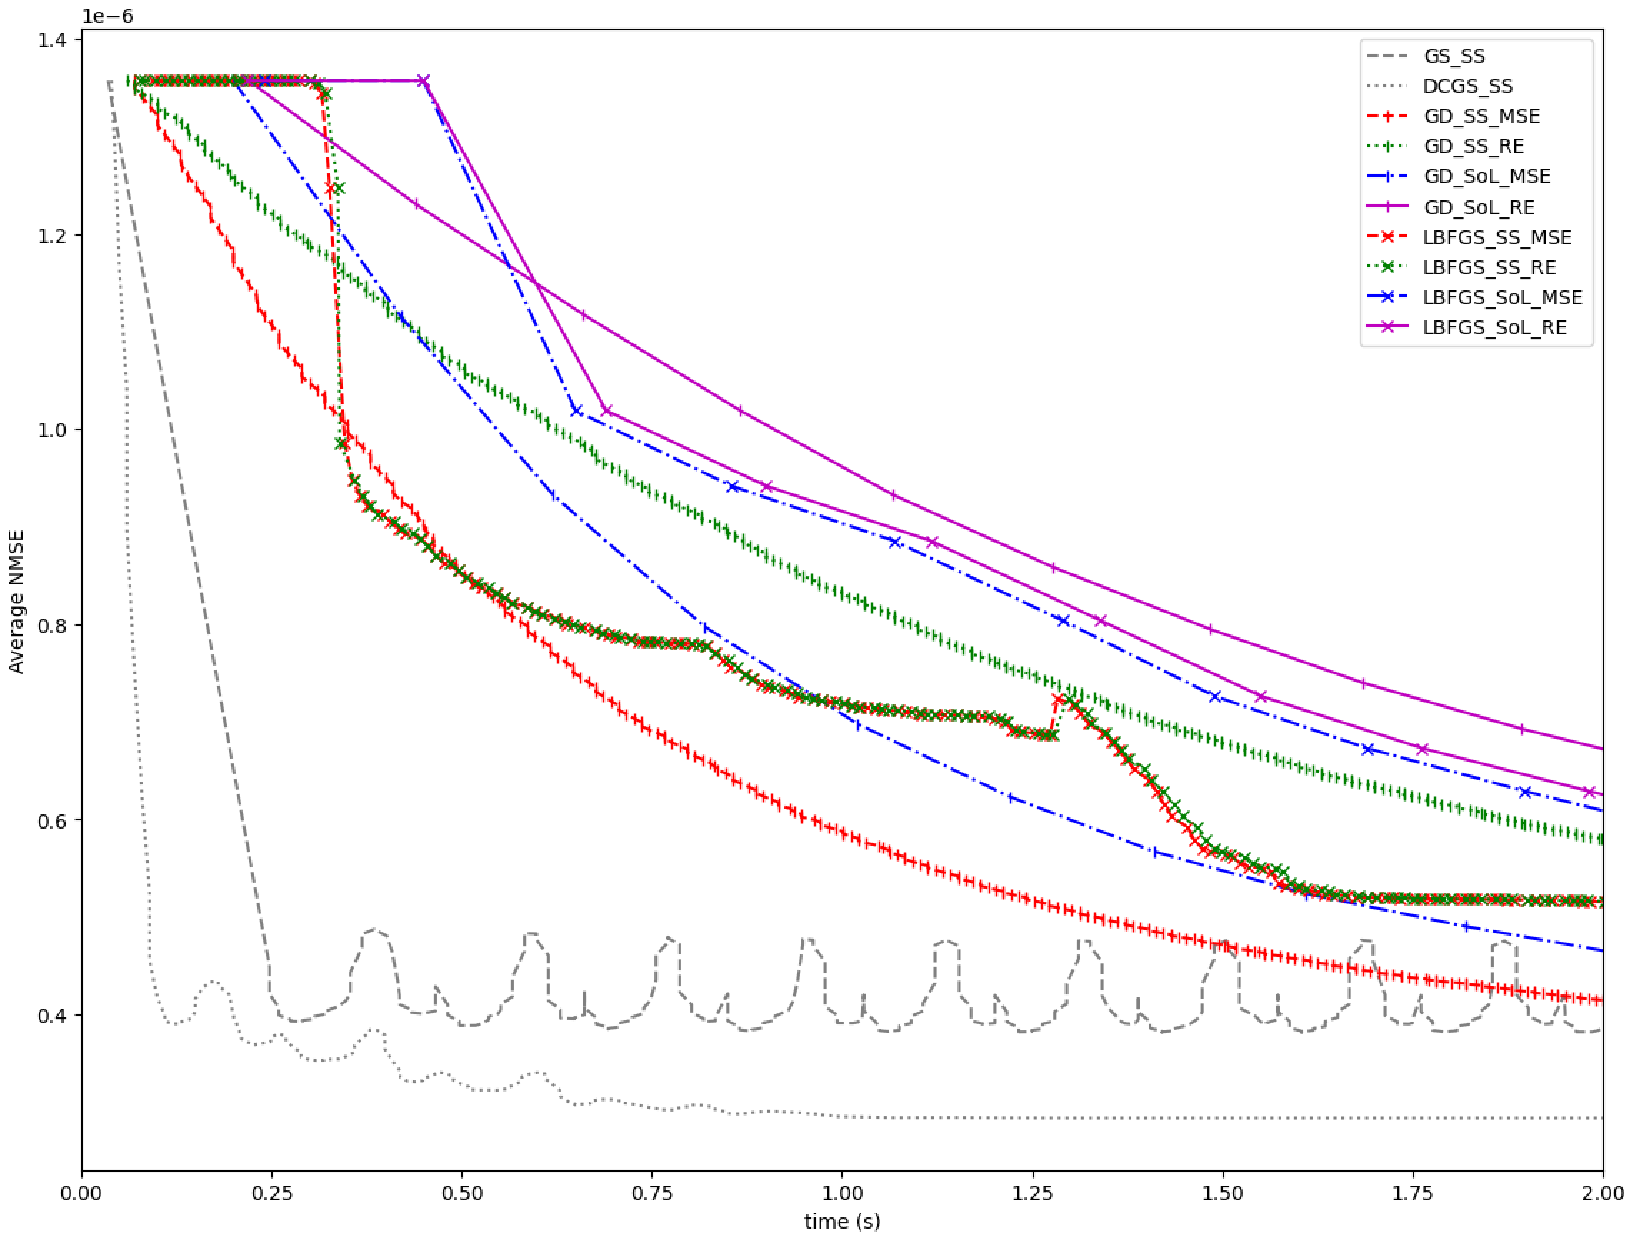
\includegraphics[width=1.0\textwidth]{Teapot_Average_NMSE_vs_time}
	\caption{Average NMSE v.s. time plot for the 30-slice target}
	\label{fig:Teapot_Average_NMSE_vs_time}
\end{figure}

\begin{figure}[H]
	\centering
	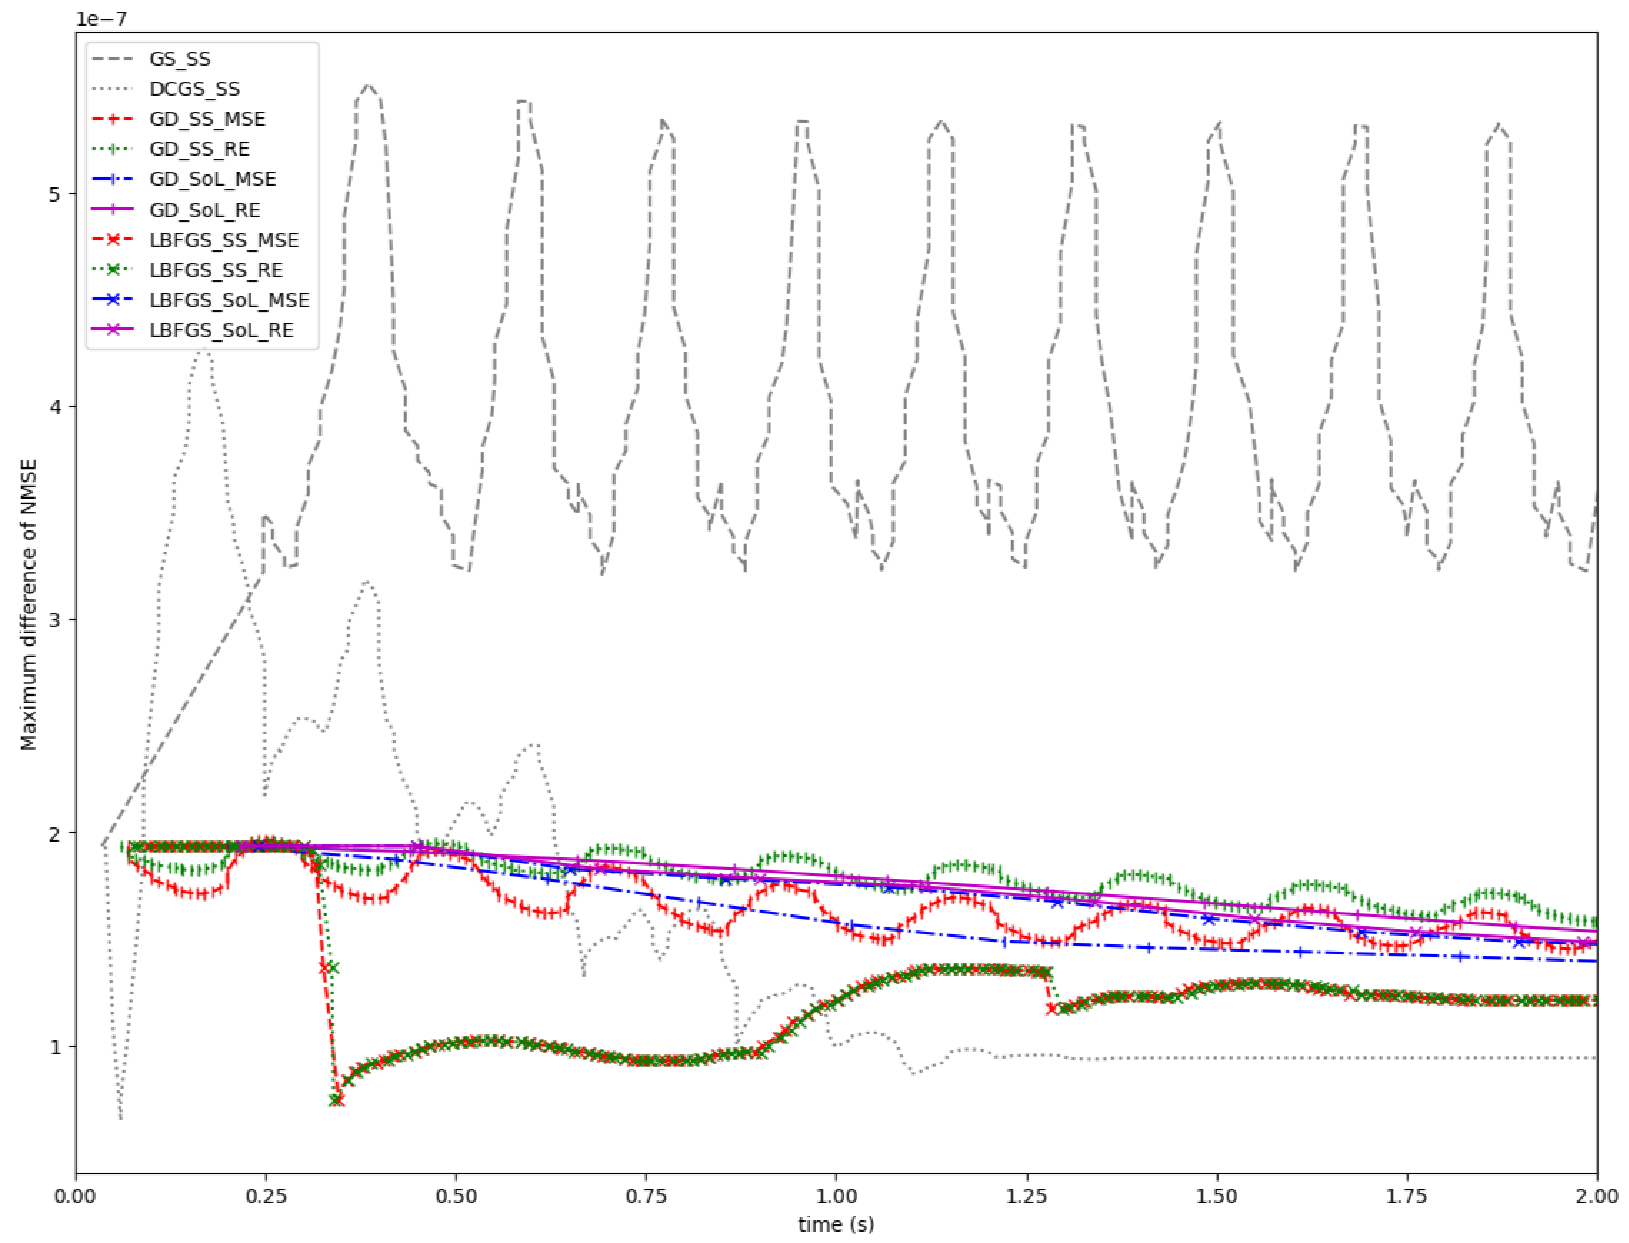
\includegraphics[width=1.0\textwidth]{Teapot_Max_diff_NMSE_vs_time}
	\caption{Difference between the maximum and minimum NMSE across all slices v.s. time plot for the 30-slice target}
	\label{fig:Teapot_Max_diff_NMSE_vs_time}
\end{figure}

\cref{fig:Teapot_Average_NMSE_vs_time} shows that, for both GD and L-BFGS optimisation algorithms, the SS technique is faster than the SoL technique. Among the SS techniques, GD, GS and DCGS algorithms achieved less average NMSE than the proposed L-BFGS with SS method, but from the maximum difference of NMSE plot in \cref{fig:Teapot_Max_diff_NMSE_vs_time}, it can be shown that the L-BFGS algorithm has less quality imbalance than the GD algorithm and the GS algorithm, although admittedly it is not as good as the DCGS algorithm. Nevertheless, the proposed method has achieved an improvement of phase retrieval using optimisation algorithms, in speed and quality imbalance suppression.


%%%%%%%%%%%%%%%%%%%%%%%%%%  Conclusion  %%%%%%%%%%%%%%%%%%%%%%%%%%
\subsection{Summary}
This chapter has proposed the method of using L-BFGS optimiser with SS technique to generate phase-only hologram for multi-depth target. The L-BFGS with SS technique has demonstrated a good suppression on the quality imbalance across the multi-depth slices, benefiting from the nature of L-BFGS being a second order optimiser, which implicitly records the historical gradients by other slices for the determination of the descent direction. For both GD and L-BFGS optimisation algorithms, the SS technique runs faster and produces better reconstruction quality than the simple SoH technique, and it is much quicker than the SoL technique especially when the number of slices get large. The proposed method has demonstrated great ability of time-limited optimisation of multi-slice 3D CGH.